\documentclass[11pt,oneside,leqno,openright]{report}
\usepackage[a4paper,width=150mm,top=25mm,bottom=25mm,bindingoffset=6mm]{geometry}

\usepackage{setspace}
\doublespacing

\usepackage[utf8]{inputenc}
\usepackage[english]{babel}

\usepackage{graphicx}
\graphicspath{{images/}}
\usepackage{float}

\usepackage{caption}
\usepackage{subcaption}

\usepackage{fancyhdr}
\pagestyle{fancy}
\fancyhead{}
\fancyhead[LO,CE]{Chapter \thechapter}
\setlength{\headheight}{14pt}
\fancyfoot{}
\fancyfoot[LE,RO]{\thepage}
\renewcommand{\headrulewidth}{0.4pt}
\renewcommand{\footrulewidth}{0.4pt}

\usepackage[artemisia]{textgreek}
\usepackage{hyperref}
\usepackage{multirow}
\usepackage{tabularx}

\usepackage{csquotes}
\usepackage[backend=bibtex]{biblatex}
\addbibresource{references.bib}

\usepackage[acronym]{glossaries}
\newacronym{acl}{ACL}{Average Chain Length}

\newacronym{ample}{AMPLE}{Ab initio Modelling of Proteins for moLEcular replacement}

\newacronym{cc}{CC}{Correlation Coefficient}

\newacronym{conkit}{ConKit}{Contact Prediction ToolKit}

\newacronym{dca}{DCA}{Direct Coupling Analysis}

\newacronym{kde}{KDE}{Kernel Density Estimate}

\newacronym{mae}{MAE}{Mean Absolute Error}

\newacronym{mfr}{MFR}{Molecular Fragment Replacement}

\newacronym{mr}{MR}{Molecular Replacement}

\newacronym{msa}{MSA}{Multiple Sequence Alignment}

\newacronym{neff}{$N_{eff}$}{Number of Effective Sequences}

\newacronym{nmr}{NMR}{Nuclear Magnetic Resonance}

\newacronym{pdb}{PDB}{Protein Data Bank}

\newacronym{pdbtm}{PDBTM}{Protein Data Bank of Transmembrane Proteins}

\newacronym{rio}{RIO}{Residue-Independent Overlap}

\newacronym{rmsd}{RMSD}{Root Mean Square Deviation}

\newacronym{tmscore}{TM-score}{Template-Modelling score}



\makeglossaries

% \title{Thesis Title}
% \author{Felix Simkovic}
% \date{31 July 2018}

\begin{document}

% \begin{titlepage}
    \begin{center}
        \vspace{1cm}
        
        
\includegraphics[width=0.8\textwidth]{uol_logo.png}
        
        \vspace{1cm}

        \Huge
        \textbf{Covariation-derived residue contacts in \textit{ab initio} modelling and Molecular Replacement}
        
        \vspace{1.5cm}
        
        \huge
        \textbf{Felix Simkovic}

        
        \vfill

        \Large
        Thesis submitted in accordance with the requirements of the \\
        University of Liverpool\\
        for the degree of\\
        Doctor in Philosophy
        
        \vspace{1.0cm}

        September 2018

        \vspace{1.0cm}
        
        \Large
        Institute of Integrative Biology\\
        University of Liverpool\\
        United Kingdom
        
    \end{center}
\end{titlepage}

%
% \begin{center}
    \Large
    \textbf{Covariation-derived residue contacts in \textit{ab initio} modelling and Molecular Replacement}
    
    \vspace{0.5cm}
    \textbf{Felix \v{S}imkovic}
    \vspace{0.5cm}
\end{center}

This thesis is concerned with the application of predicted residue contacts in \textit{ab initio} protein structure prediction and Molecular Replacement.

% Chapter 3
The initial work in this thesis explored the use of predicted residue contacts to improve \textit{ab initio} protein structure predictions, which were used to generate ensemble search models for Molecular Replacement in AMPLE. The results proved highly encouraging. Five additional targets were tractable where previous AMPLE attempts would have been unable to achieve structure solution. In particular, the improved decoy quality appeared to be the main reason for the extended target tractability.

% Chapter 4
Following on from the initial proof-of-concept study, different contact predictions and ROSETTA energy functions were trialled to identify the optimal strategy to generate decoys for unconventional Molecular Replacement in AMPLE.

% Chapter 5
% Chapter 6
% Chapter 7



%
% \chapter*{Dedication}
% To mum and dad
%
% \chapter*{Declaration}
% I declare that..
%
% \chapter*{Acknowledgements}
% I want to thank...

\tableofcontents

% \listoffigures
%
% \listoftables

\printglossary

\chapter{Introduction}
% 
%
% X-ray crystallography
%

\section{Macromolecular X-ray crystallography}
The discovery of X-ray diffraction by crystals by Max van Laue \cite{Friedrich1913-vx,Laue1913-sn} marked the origins of modern crystallography. However, it was not until the work of William Lawrence Bragg and William Henry Bragg that X-ray scattering could be interpreted as atomic positions \cite{Bragg1913-cx,Bragg1929-xp,Bragg1912-ht}. Since then, X-ray crystallography and the determination of atomic positions in organic and inorganic molecules has come a long way and shaped the path for many 21\textsuperscript{st} century discoveries. Amongst those groundbreaking discoveries are the earliest structural models of biological molecules including DNA \cite{Watson1953-qw}, vitamin B12 \cite{Hodgkin1956-mx}, and the first protein structures \cite{Blundell1971-mv,Blake1965-ng,Perutz1960-qz,Kendrew1958-on}. These structure elucidations hallmarked the dawn of a new era in biological and biomedical research. At the time of writing, 124,551 structural models deposited in the \gls{pdb} were determined by X-ray diffraction studies \cite{Berman2000-ua}, and thus X-ray crystallography is a key method in biological research.

\subsection{X-ray scattering}
X-rays are high energy photons part of the electromagnetic spectrum with a wavelength 0.1-100\AA\ \cite{Rupp2010-nc}. X-rays can be described as packets of travelling electromagnetic waves, whose electric field vector interacts with the charged electrons of matter \cite{Rupp2010-nc}. Such interaction, typically termed scattering, results in the diffraction of the incoming wave, which X-ray crystallography relies on.

In its simplest form, scattering of X-ray radiation can be explained in the scenario of exposure to a single free electron. The resulting scattering can be classed as elastic (Thomson scattering) or inelastic (Crompton scattering) \cite{Rupp2010-nc}. The latter --- scattering that results in a loss of energy of the emitting photon due to energy transfer onto the electron --- does not contribute to discrete scattering, the type of scattering X-ray diffraction relies on. In comparison, Thomson scattering does not result in a loss of energy of the emitting photon. This has significant effects, the incoming photon emits with the same frequency causing the electron to oscillate identically further enhancing the signal.

\begin{figure}[H]
    \centering
    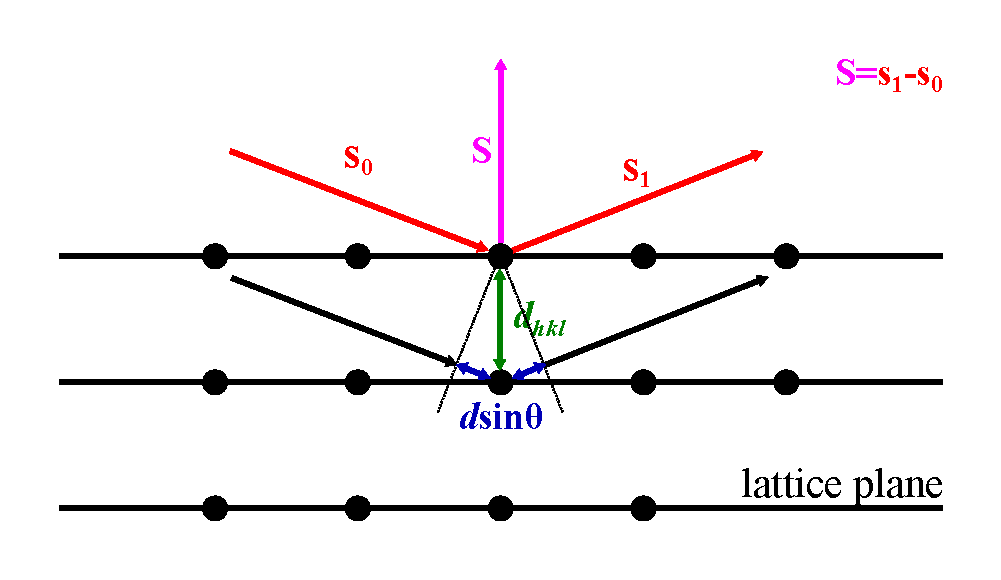
\includegraphics[width=0.7\textwidth]{introduction_bragg.pdf}
    \caption{Schematic of Bragg scattering.}
    \label{fig:introduction_bragg}
\end{figure}

If we expand the example to include all electrons in an atom and expose the atom to X-ray radiation, our theory needs to be slightly expanded. Given that one or more electrons in an atom are not free but orbit around the atom's nucleus in a stable and defined manner, the distribution of these electrons around the nucleus determines the scattering of the incoming X-ray photons. The distribution of scattered photon waves is thus an overall representation of the probability distributions of each electron in the atom and is referred to as electron density $\rho(\boldsymbol{r})$. In X-ray scattering, it suffices to approximate the shape of the electron density to a sphere. If we now consider the emitting wave $\boldsymbol{s_1}$ of an X-ray photon scattered by any position $\boldsymbol{r}$ in the electron density of an atom, then the phase difference $\Delta\varphi$ to the incoming wave $\boldsymbol{s_0}$ can be described by \cref{eq:phase_difference} \cite{Rupp2010-nc}.

\begin{equation}
    \Delta\varphi=2\pi\left(\boldsymbol{s_1}-\boldsymbol{s_0}\right)\boldsymbol{r}=2\pi \cdot \boldsymbol{S}\boldsymbol{r}
    \label{eq:phase_difference}
\end{equation}
\equations{Phase difference equation}

If more than one electron in an atom's electron density scatter the incoming X-ray photon wave, then the emitting partial waves can be described by the atomic scattering function $f_s$ (\cref{eq:atomic_scattering_factor}), which describes the interference of all scattered waves \cite{Rupp2010-nc}. The total scattering power of an atom is proportional to the number of electrons and element-specific with heavier atoms scattering more strongly. Given the approximation of a centrosymmetric electron density, the atomic scattering function is also symmetric.

\begin{equation}
    f_s=\int\limits_{\boldsymbol{r}}^{V(atoms)}\rho\left(\boldsymbol{r}\right) \cdot \exp\left(2\pi\\i\boldsymbol{S}\boldsymbol{r}\right) \cdot d\boldsymbol{r}
    \label{eq:atomic_scattering_factor}
\end{equation}
\equations{Atomic Scattering Factor equation}

With an enhanced understanding of X-ray scattering of electrons orbiting a single atom, it is important to consider X-ray scattering of adjacent atoms, such as it is typically found in molecules. If the electromagnetic wave of a X-ray photon excites all electrons of adjacent atoms, then the resulting partial waves --- amplified by oscillations of electrons of Thomson scattering --- result in constructive or destructive interference. Maximal interference can be obtained when all partial waves are in phase, and maximal destructive interference when out-of-phase. This leads to varying intensities of the emitting X-ray photon at different points in space. To obtain the overall scattering power $F_s$ of all contributing atoms, \cref{eq:atomic_scattering_factor} needs to be modified to include the sum over all atoms $j$ as described in \cref{eq:total_scattering_power}.

\begin{equation}
    F_s=\sum_{j=1}^{atoms}f_{s,j}^0 \cdot \exp\left(2\pi\\i\boldsymbol{S}\boldsymbol{r}_j\right)
    \label{eq:total_scattering_power}
\end{equation}
\equations{Total Scattering Power equation}

If we now translate our hypothetical experiment into a crystal lattice then our understanding described in \cref{eq:total_scattering_power} needs to be expanded from a 1-dimensional distance vector $\boldsymbol{r}$ to the three dimensional lattice translation vectors $\boldsymbol{a}$, $\boldsymbol{b}$ and $\boldsymbol{c}$. The Laue equations (\cref{eq:laue_equations}) do exactly that and ultimately determine the positions of the diffraction peaks in 3-dimensional space.

\begin{equation}
    \boldsymbol{S} \cdot \boldsymbol{a}=n_1, \quad \quad \boldsymbol{S} \cdot \boldsymbol{b}=n_2, \quad \quad \boldsymbol{S} \cdot \boldsymbol{c}=n_3
    \label{eq:laue_equations}
\end{equation}
\equations{Laue equations}

Such determination is possible through the findings made by \textcite{Bragg1913-cx}, who identified the relationship between the scattering vector $\boldsymbol{S}$ and the planes in the crystal lattice. Today, this relationship is defined by the Bragg equation (\cref{eq:bragg_equation}) \cite{Bragg1913-cx}, which allows us to interpret X-ray diffraction as reflections on discrete lattice planes, which relates the diffraction angle $\theta$ to the lattice spacing $d_{hkl}$ (\cref{fig:introduction_bragg}) \cite{Rupp2010-nc}. For maximum diffraction $n$ needs to be an integer multiple to result in maximum constructive interference of wavelength $\lambda$.

\begin{equation}
    n\lambda=2d_{hkl}sin\theta
    \label{eq:bragg_equation}
\end{equation}
\equations{Bragg equation}

If the hypothetical model is expanded to molecular crystals, then the total scattering from the unit cell is merely a summation of all molecular unit cell scattering contributions in the crystal. Mathematically, this results in \cref{eq:total_scattering_power} being generalised to \cref{eq:structure_factors} through the application of the Laue equations (\cref{eq:laue_equations}). This allows us to express the scattering vector $\boldsymbol{S}\boldsymbol{r}_j$ as Miller indices of the reflection planes $\boldsymbol{h}\boldsymbol{x}_j$.

\begin{equation}
    F_h=\sum_{j=1}^{atoms}f_{s,j}^0 \cdot \exp\left(2\pi\\i\boldsymbol{h}\boldsymbol{x}_j\right)
    \label{eq:structure_factors}
\end{equation}
\equations{Mathematical expression of a Structure Factor}

The structure factor equation defines the scattering power from a crystal in a given reciprocal lattice direction $\boldsymbol{h}$. The scattering is enhanced by the number of repeating units of lattice translation vectors $\boldsymbol{a}$, $\boldsymbol{b}$ and $\boldsymbol{c}$, and thus the overall scattering power is proportional to the number of unit cells in the crystal.

It should be noted that \cref{eq:structure_factors} is a simplification of the problem at hand. In reality, instrument and experimental corrections need to be applied to the structure factor equation. A correction factor for each experiment-dependent parameter needs to be applied to the structure factor equation. However, in the scope of this work the details of such correction factors do not need to be discussed.

Since complex structure factors describe the molecular structure in the reciprocal space domain, the conversion to the real space domain in form of electron density is required. This can be conveniently done through the bijective Fourier transform, which allows the conversion of complex structure factors to electron density and vice versa without the loss of any information \cite{Rupp2010-nc}. Thus, electron density can be obtained from the complex structure factors using \cref{eq:electron_density}. The normalisation factor $1/V$ ($V$ represents the volume of the unit cell) provides the correct units for the electron density $\rho(x,y,z)$.

\begin{equation}
    \rho(x,y,z)=\frac{1}{V}\sum_{h=0}^{+\infty}\sum_{k=-\infty}^{+\infty}\sum_{l=-\infty}^{+\infty}\boldsymbol{F}(hkl)\cdot \exp\left(-2\pi\\i(hx+ky+lz)\right)
    \label{eq:electron_density}
\end{equation}
\equations{Mathematical expression of Electron Density}

\subsection{From crystal to structure}
In X-ray crystallographic experiments, X-ray radiation is measured using light detectors. However, the measurement taken is incomplete. Light detectors only capture the intensity of the scattered X-ray photons but crucially lose the phase information. The latter is essential for atomic reconstruction of the crystallised molecule, and thus needs to be obtained. In \gls{mx}, experimentalists have a number of alternative techniques to compensate for the lost phase information. 

Prior to the big advances in computing power and the successful elucidation of many protein structures, \gls{mx} crystallographers primarily recovered the lost phase information through Direct Methods or Experimental Phasing \cite{Rupp2010-nc}. Today, the most popular method to recovering the lost phase information is \gls{mr} \cite{Rossmann2001-yw,Rossmann1990-am}. In a \Gls{mr} search, a known structure (`search model') similar to the unknown is relocated in the unit cell until the solution with the best fit between calculated and observed diffraction data is obtained \cite{Rupp2010-nc}. A 6-dimensional search, i.e. a simultaneous rotation and translation search, is possible \cite{Kissinger1999-ho,Glykos2000-gc,Read2001-nu}, but is computationally very expensive and less suitable for challenging cases. In comparison, most modern crystallographic applications opt for two distinct sub-searches, the rotation search to orient the search model within the unit cell followed by the translation search to locate it \cite{Rupp2010-nc}. The benefits over a combined search include search-specific target functions that enable increased sensitivity and additional terms to compensate for imperfect data. 

The most successful \gls{mr} algorithms perform the rotation and translation searches using Patterson methods or Maximum Likelihood functions. Patterson methods --- originally developed by \textcite{Rossmann1962-ou} --- rely on the use of a map of vectors between the scattering atoms, which can be determined for the calculated and observed structure factor amplitudes. Patterson vectors can be sub-classed as intra- and inter-molecular vectors. A distinct separation of the observed vectors is impossible. However, inter-molecular vectors appear further away from the central peak of self-vector (vector from atom to itself) in the Patterson map \cite{Rupp2010-nc}. The calculated Patterson vectors for the search model allow for a clearer distinction between the intra- and inter-molecular vectors. If the search model is placed in a large unit cell, then inter-molecular vectors must scale with the unit cell dimension \cite{Rupp2010-nc}. Ultimately, using the intra-molecular Patterson vectors, the search model can be oriented against the experimentally determined Patterson vectors. In a similar manner, the inter-molecular vectors can be used to identify the correct translation of the search model. Patterson methods are very sensitive to small orientation errors of the search model \cite{Rupp2010-nc}. Thus, orientations with the highest vector peak overlaps are trialed in the subsequence translation search. Given that Patterson methods operate by Patterson vector comparisons in rotation and translation searches, these methods do not require search-model-derived phases.

In comparison to the Patterson methods, Maximum Likelihood methods do not rely on inter-atomic vectors in Patterson maps. Instead, Maximum Likelihood methods make use of Bayes' theorem \cite{Bayes1763-ox} to compare calculated structure factors and observed structure factor amplitudes directly \cite{Read2001-nu}. Bayes' theorem in crystallographic Maximum Likelihood methods is applied to compute the likelihood that an experimental value is observed given the current search model. The maximal likelihood indicates the best search model given the observed experimental data. Since the search model likelihood term is the product of many individual probabilities, which are difficult to represent computationally due to floating point representations, the log of the likelihood is commonly used \cite{Rupp2010-nc}. The major advantage of Maximum Likelihood methods over Patterson methods centres on the more realistic target functions, which consider errors and incompleteness of the search model, apply bulk solvent correction and conduct multi-model searches \cite{Read2001-nu}. The latter is of particular relevance since the Maximum Likelihood rotation function can thus consider already placed search models in a fixed position whilst trialling additional ones \cite{Storoni2004-ed}, which proves to be a major advantage over Patterson methods.  Furthermore, likelihood target functions can consider the structural variance of multiple superposed models in an ensemble search model, which is used to weight structure factors at the various positions to improve the overall likelihood term \cite{Read2001-nu}. 

The initial electron density map --- regardless of its determination by \gls{mr} or Experimental Phasing --- is almost always inaccurate. In \gls{mr}, inaccuracies arise from experimental errors, model incompleteness, low signal-to-noise or model bias. Thus, approaches for improving the phases used to calculated the initial electron density map have been developed and are routinely applied in \gls{mx}. \textit{Density modification} describes a set of methods that improve the obtained electron density typically by applying statistical corrections to electron density distributions. These corrections are based on prior knowledge or assumptions of the physical properties of macromolecular structures \cite{Rupp2010-nc}. This process can transform initially poor or uninterpretable initial electron density maps to high quality ones. Three predominant density modification approaches exist: solvent flattening, histogram matching and the ``sphere-of-influence'' method. Solvent flattening is an approach first proposed by \textcite{Wang1985-zu}, which exploits the fact that solvent regions in protein crystals are disordered, and thus differ in electron density from macromolecule-containing regions. If solvent electron density is set to a constant, then it is essentially flattened which will result in improved structure factors with improved phases and thus improved electron density. Histogram matching \cite{Lunin1988-lx} exploits the defined characteristics of an electron density distribution determined from sets of proteins at the same resolution, irrespective of individual structural details. The electron density distribution for noisy maps are Gaussian-shaped. In contrast, the electron density distribution of a feature-defined map is positively skewed. Thus, attempting to improve the Gaussian-shaped electron density distribution to better match the positively skewed shape results in overall improvements to the electron density. The ``sphere-of-influence'' method was introduced by \textcite{Sheldrick2002-tx} and classifies solvent and protein electron density by observing its variance across the shell surface of a 2.42\AA\ sphere (dominant 1-3 atom distance in macromolecular structures). If the sphere is positioned in the disordered solvent region typically found in inter-molecular channels, the density variance will be low. Thus, this approach allows to smoothen solvent-containing regions of the electron density \cite{Sheldrick2002-tx}. Independent of the density modification strategy applied, it is important to understand that improvements to the electron density map anywhere lead to improvements everywhere by transferral of information from one part of the map to another \cite{Terwilliger2000-sz}.

A second approach to improving the initial electron density is termed \textit{refinement}. Iteratively, the placed search model is optimised to better explain the experimentally observed data. This optimisation problem is typically broken down into three main steps: the definition of the model parameters, the scoring function and the optimisation method. The model parameters describe the crystal and its content and can be subdivided into atomic and non-atomic model parameters \cite{Afonine2012-bg}. These parameters combined are used to score the current model. The scoring function relates the experimental data to the model parameters. The scoring function contains two primary terms, the refinement data target and an \textit{a priori} knowledge term. The former defines a target function that assesses the similarity between calculated and experimental structure factors. The target function is commonly a Maximum Likelihood-based function that considers missing or incomplete data \cite{Murshudov2011-ww,Afonine2012-bg}. The \textit{a priori} knowledge term in the scoring function defines the properties of a good model by including stereochemical property terms. Lastly, optimisation methods provide tools to vary the model parameters to better fit the experimental data. Different optimisation techniques can be used depending on the severity of model parameter alteration, which generally depend on the entrapment of states in local energy minima. Model parameterisation and its scoring against the pre-defined scoring function combined with model optimisation form a refinement macrocycle, which is iteratively used to optimise a model's fit to the experimental data. This ultimately improves both the electron density map interpretability and model quality. \gls{mx} refinement can be performed in structure-factor-based reciprocal space and electron-density-based real space \cite{Afonine2012-bg}. A combination allows global and local refinement strategies and enables grid-like searches to optimise the model parameters until convergence.

Once initial phase information is improved through refinement and/or density modification, attempts can be made to build atomic model coordinates into the electron density map. This process is typically coupled with refinement or density modification to iteratively improve the quality of the partially built model and the electron density map \cite{Rupp2010-nc}. A small number of distinct algorithms are currently used to automatically build atomic coordinates into electron density: main-chain autotracing \cite{Sheldrick2010-cx}, fitting pseudo-atoms into electron density \cite{Lamzin2001-cn}, or fitting reference coordinates with similar electron density maps \cite{Terwilliger2004-ig,Cowtan2006-xv}. In essence, all algorithms attempt to maximise the number of correctly identified and placed atomic coordinates into available electron density. Whilst autotracing solely builds main-chain polypeptides, the other two approaches rely on sequence information to also build side-chains. Independent of the complexity of the model building task, the higher the resolution and the more complete the initial starting model, the less ambiguous and challenging this task becomes \cite{Rupp2010-nc}. 

\subsection{Unconventional Molecular Replacement}
The process of macromolecular structure determination via conventional \gls{mr} has been outlined previously. Search models are typically derived from structural homologs identified by sequence identity to the crystallised target \cite{Rupp2010-nc}. However, homologous structures are not always available or impossible to identify by current approaches. Experimental phasing approaches to circumvent the absence of \gls{mr} templates can be expensive, unsuccessful and very challenging for certain protein targets, and thus remain infeasible to pursue at times. Under such circumstances, alternative approaches are required, which are referred to as ``unconventional'' \gls{mr} approaches from here onwards. The unconventional \gls{mr} approach most relevant to the work presented in this thesis utilises the 3-dimensional structure prediction of a protein target starting from its sequence \cite{Qian2007-vo,Rigden2008-vo,Das2009-uz}. Although two distinct methods exist to predict the protein structure of a target sequence, homology modelling and ab initio structure prediction, only the latter is relevant to this work since the former relies on homologous structures.
 
%
% Structure prediction
%

\section{\textit{Ab initio} protein structure prediction} \label{sec:introduction_structure_prediction}
The folding of protein structures is commonly described by the folding funnel hypothesis \cite{Leopold1992-yf}. It assumes that the native state of a protein fold corresponds to its global minimum free energy state along its energy surface (\cref{fig:introduction_foldingfunnel}) \cite{Anfinsen1973-in}. \textit{In silico} protein folding experiments attempt to find this lowest-free-energy state of the protein fold. However, to unambiguously identify it sampling of all polypeptide chain conformations is necessary. In theory, sampling of all conformations for a 100-residue protein takes in the order of approximately $10^{52}$ years ($10^7$ configurations with $10^{-11}$ seconds per configuration), yet \textit{in vivo} an equivalent polypeptide chain folds in milliseconds to seconds \cite{Levinthal1969-bn,Karplus2011-jh}. This paradox --- termed the Levinthal paradox \cite{Levinthal1969-bn} --- created the basis for the folding funnel hypothesis.  

\begin{figure}[H]
    \centering
    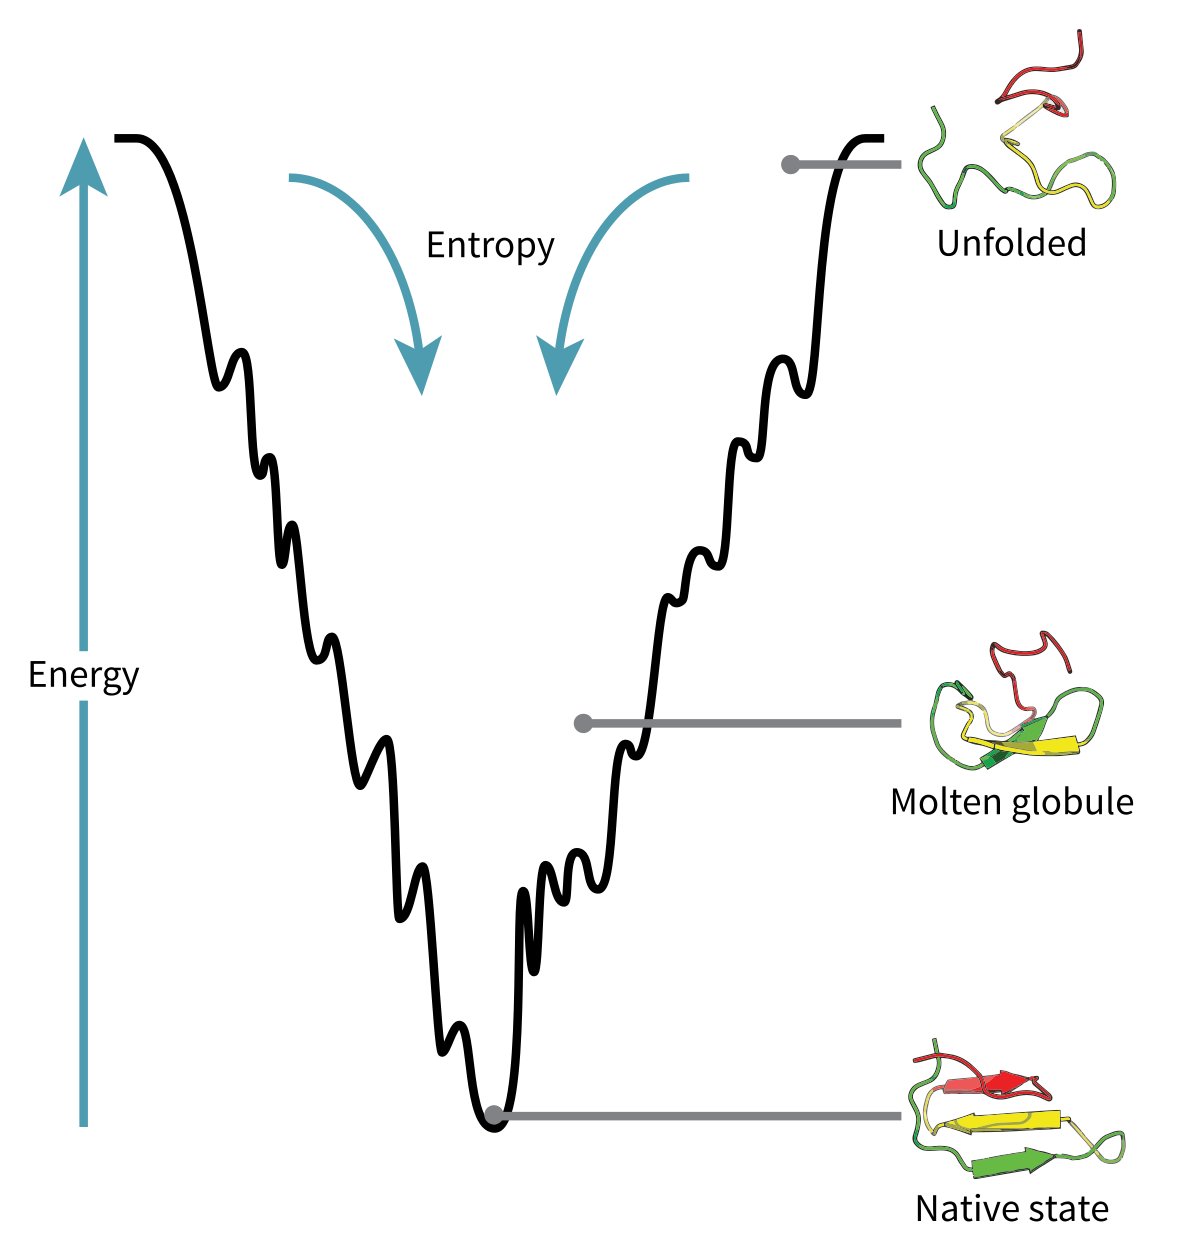
\includegraphics[width=0.5\textwidth]{introduction_foldingfunnel.png}
    \caption[Schematic of the folding funnel hypothesis.]{Schematic of the folding funnel hypothesis \cite{Leopold1992-yf}. Diagram produced by \textcite{Wikipedia-FoldingFunnel} contributors.}
    \label{fig:introduction_foldingfunnel}
\end{figure}

In \textit{ab initio} protein structure prediction, the tertiary structure of a protein is predicted using its primary structure alone. This problem is in its nature identical to finding the lowest-energy state along a protein's energy landscape. However, in an attempt to avoid the Levinthal paradox, different knowledge- and physics-based energy functions coupled with a variety of conformational-search sampling algorithms are employed \cite{Lee2017-oc}. 

Physics-based energy functions use physiochemical force fields typically coupled with Molecular Dynamics simulations to sample the folding trajectory of a protein sequence (true physics-based approaches are computationally intractable because quantum mechanics models would need to be used). Force fields describe parameter sets used to calculate energy potentials for a system of atoms in a simulation run, and include potentials such as van der Waals and electrostatic interactions \cite{Lee2017-oc}. In the context of \textit{ab initio} protein structure prediction, pure physics-based approaches are often less favourable, because the computational complexity to find the lowest free-energy state of a large protein structure remains intractable without the use of supercomputers.

Knowledge-based energy functions rely on empirical energy terms derived from statistics and regularities of experimentally determined structures \cite{Lee2017-oc}. These energy terms can be subdivided into two types, the generic or sequence-independent terms and amino-acid or sequence-dependent terms \cite{Skolnick2006-uv}. The former include terms to describe the backbone hydrogen-bonds and local backbone stiffness of a polypeptide chain. The sequence-dependent terms include terms such as pairwise residue contact potential, distance-dependent atomic contact potential, and secondary structure propensities. However, predicting local or global tertiary structure of a protein sequence using empirical energy terms alone is very difficult. Subtle differences in the local and global environment of a primary structure alongside the subtle differences in initial folds leading to common secondary structure features are very difficult to reproduce in a modelling scenario. Thus, knowledge-based energy functions are often coupled with the assembly of fragments extracted from other protein structures to predict the unknown tertiary structure of the target sequence \cite{Lee2017-oc}. 

The most successful \textit{ab initio} structure prediction protocols use knowledge-based and physics-based energy functions combined with fragment-assembly-based conformational searches to find the lowest free-energy state \cite{Rohl2004-dj,Xu2012-jf,Blaszczyk2013-nx,Kosciolek2014-bt,De_Oliveira2017-sg}. Structural fragments of varying lengths (typically 3-20 residues) are extracted from existing protein structures \cite{Abbass2015-qk,Shen2013-wh,Li2008-xu,Kalev2011-sz,Bhattacharya2016-ix,Wang2017-ka,De_Oliveira2015-kb,Gront2011-sv}. These fragments are used in a Monte Carlo simulation to search the conformational space of the polypeptide chain for low free-energy states \cite{Metropolis1949-kp}. The insertion of overlapping fragments results in the replacement of torsion angles either at random positions or sequentially from pre-defined starting position (such as N- or C-termini), and each move is scored against the Metropolis criterion \cite{Metropolis1949-kp} consisting of knowledge-based and physics-based terms. The Metropolis criterion is typically defined to accept fragment insertions that lower the free-energy term of a decoy, whilst sometimes accepting insertions that increase the free-energy term to escape local energy minima. If the insertion of a fragment passed the Metropolis criterion, the related torsion angles are accepted and integrated in the polypeptide chain for the next fragment-insertion iteration. This process is repeated until convergence of the decoy, i.e. no lower free-energy state can be found. In all routines, these steps are independently repeated thousands of times to create a pool of decoys. 

In order to identify the correct fold amongst the thousands of generated decoys, clustering approaches are often used in combination with \textit{ab initio} protocols. \textcite{Shortle1998-fq} identified that the most-similar decoy to the native structure is most often the centroid (decoy with most neighbours in the cluster) of the largest cluster. Further studies showed that the selection of those centroid decoys helps to identify the most native-like folds amongst the many thousands generated \cite{Zhang2004-uz,Bradley2005-lw,Oldziej2005-qp}. Some protocols use clustering as an intermediate or final step to identify decoys for which it will perform more computationally demanding all-atom refinement \cite{Bradley2005-lw} or other decoy hybridisation techniques \cite{Zhang2004-uc,Xu2012-jf,Yang2015-oc} to further approach the native-like fold \cite{Kryshtafovych2016-aq}.

Despite active research in \textit{ab initio} protein structure prediction over decades, all approaches struggle with accurate predictions for larger protein domains (chain lengths $>150$ residues) \cite{Bradley2005-lw,Tai2014-rz,He2013-gm,Kinch2011-py}. The major challenge arises from the sampling of the conformational space since incorrect local changes influence the global structure. Furthermore, \textbeta-sheets are inherently difficult to predict given that \textbeta-strands in fragment-based approaches are inserted one at a time yet rely on the hydrogen-bond network typically found in \textbeta-sheets to reduce the overall energy of the decoy. To address this issue, \textcite{Lange2012-yh,Raman2010-xv,Gobl2014-gc} started to use \gls{noe} data as residue-residue distance restraints to reduce the sampling space of conformations, which enabled high-resolution predictions of tertiary structure for longer proteins. Although successfully applied in the aforementioned examples, experiments to collect \gls{noe} data are costly, challenging and intractable for larger multi-domain targets. To avoid this problem yet obtain similarly useful information on spatial proximity of amino acids in a protein fold, researchers started to exploit residue-residue contact information, which enables accurate \textit{ab initio} structure prediction for longer polypeptide chains (e.g., \cite{Marks2011-os,Michel2014-eg,Kosciolek2014-bt,Ovchinnikov2015-tn,Ovchinnikov2016-jj,Michel2017-xh,De_Oliveira2017-sg,Ovchinnikov2017-nd,Wang2017-rx}).

%
% Contact predition
%

\section{Residue-residue contact prediction} \label{sec:introduction_contact_prediction}
The use of residue-residue contact information to reduce the conformational search space in protein structure prediction relies on accurate identification of amino acids in close spatial proximity. Today, such identification can be detected from sequence information alone by either \gls{dca} or \gls{sml} algorithms.

\subsection{Direct Coupling Analysis}
\Acrlong{dca} uses protein sequence information to identify coordinated changes of amino acids in sequences of a protein family (\cref{fig:introduction_covariance}). These coordinated changes are caused by evolutionary pressure to maintain residue interactions important for protein structure and function. However, original attempts to detect covariation signal from sequences in a protein family were unsuccessful for many years \cite{Taylor1994-es,Gobel1994-rp,Neher1994-qn,Shindyalov1994-yp}. The applied local statistical model suffered from numerous drawbacks, including the loss of covariation signal due to phylogenetic dependencies, limited availability of sequence data, and the potentially false assumption that truly coevolved residues are in close proximity in sequence space \cite{Pollock1997-os,Lapedes1999-cg,Lapedes2012-tu}. Implementations of the local statistical model used raw covariation frequencies between pairs of positions in the sequence alignment. This further poses issues since successful distinction between ``direct'' casual (A-B and B-C) and ``indirect'' transitive (A-C) correlations is essential for successful protein structure prediction yet cannot be separated by frequency comparisons. 

\begin{figure}[H]
    \centering
    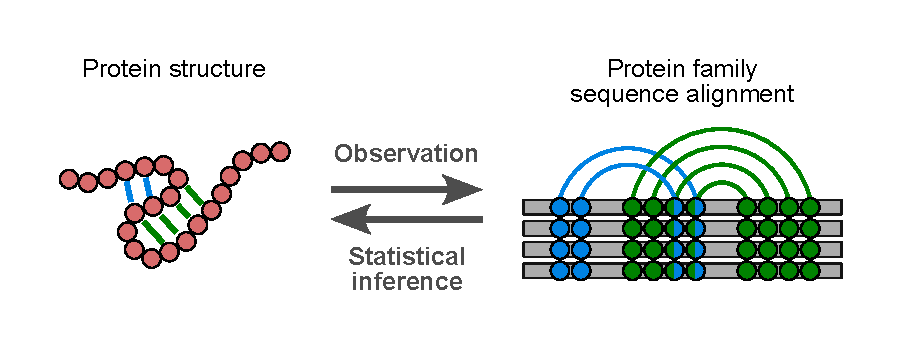
\includegraphics[width=1.0\textwidth]{introduction_covariance.pdf}
    \caption[Schematic of inference of covariance signal]{Schematic of inference of covariance signal originating from evolutionary pressure in protein tertiary structures and encoded in its family's sequence alignment (adapted from \cite{Simkovic2017-xs}).}
    \label{fig:introduction_covariance}
\end{figure}

\textcite{Lapedes1999-cg} proposed the use of a global statistical model to infer correlations of residue pairs to circumvent the main problem of decoupling causal and transitive correlations. However, it was not until a decade later before first implementations of the global statistical model surfaced to successfully disentangle these types of correlations \cite{Weigt2009-sx,Burger2010-ee,Balakrishnan2011-wh,Marks2011-os,Morcos2011-lk,Jones2012-ks,Ekeberg2013-ay,Kamisetty2013-le,Seemayer2014-zp}. Global statistical models achieve successful disentanglement by inferring a probabilistic description of the sequence alignment that best explains observed correlations using underlying causal couplings between positions \cite{Hopf2017-pp}. Such couplings can be inferred by maximising the likelihood of observing the sequences in the alignment under the maximum entropy probability model. In other words, by considering all amino acid pair positions simultaneously, causal and transitive couplings can be successfully disentangled \cite{Ekeberg2013-ay}.

The pairwise probabilistic model $P(\boldsymbol{\sigma})$ of the amino acid sequence $\boldsymbol{\sigma}=\left(\sigma_1,\sigma_2,\dots,\sigma_N\right)$ of length $N$ is defined in \cref{eq:potts_model}, which contains the amino acid configuration constraints $\sigma_i$ and $\sigma_j$ at positions $i$ and $j$, the single-site conservation bias term $h_i$, and co-conservation term $J_{ij}$ between position pairs $i,j$. 

\begin{equation}
    P(\boldsymbol{\sigma})=\frac{1}{Z}\exp\left(\sum_{i=1}^{N}h_i\left(\sigma_i\right)+\sum_{1 \leqslant i < j \leqslant N}J_{ij}\left(\sigma_i, \sigma_j\right)\right)
    \label{eq:potts_model}
\end{equation}
\equations{Potts model}

The partition function $Z$ (\cref{eq:potts_model_partition_function}) acts as normalising constant, and additionally has the property to maximise the entropy in the probabilistic model. However, the computation of $Z$ is intractable for the feature space found in \gls{dca} since the number of summations in $Z$ exponentially increases with $N$ for all 20 amino acid configurations. Thus, approximations of $Z$ are typically used, which were shown to lead to precise covariance predictions \cite{Ekeberg2013-ay}.

\begin{equation}
    Z=\sum_{\boldsymbol{\sigma}}^{ }\exp\left(\sum_{i=1}^{N}h_i\left(\sigma_i\right)+\sum_{1 \leqslant i < j \leqslant N}J_{ij}\left(\sigma_i, \sigma_j\right)\right)
    \label{eq:potts_model_partition_function}
\end{equation}
\equations{Partition function of Potts model}

Over the last decade, numerous approximations for the parameter inference of $P(\boldsymbol{\sigma})$ have been implemented, which include gradient ascent with Monte Carlo sampling \cite{Lapedes2012-tu}, message passing \cite{Weigt2009-sx}, mean-field \cite{Marks2011-os,Morcos2011-lk,Jones2012-ks,Stein2015-cw}, and pseudolikelihood maximisation \cite{Balakrishnan2011-wh,Ekeberg2013-ay,Kamisetty2013-le,Seemayer2014-zp,Hopf2015-vf}. However, it is the latter that has proven to be most successful, and is thus at the core of most widely-used applications. In pseudolikelihood maximisation \gls{dca} approaches, the full likelihood for each sequence position $i$ in $\boldsymbol{\sigma}$ across all sequences in the alignment is approximated by a product of conditional likelihoods (\cref{eq:covariance_pseudolikelihood_approximation}) \cite{Hopf2017-pp}.

\begin{equation}
    \mathcal{L}\left(\mathbf{h},\mathbf{J}\right)=\prod_{\sigma\in\Sigma}P\left(\sigma\rvert\mathbf{h},\mathbf{J}\right)\approx\prod_{i=1}^{N}P\left(\sigma_i\rvert\sigma\backslash\sigma_i,\mathbf{h},\mathbf{J}\right)
    \label{eq:covariance_pseudolikelihood_approximation}
\end{equation}
\equations{Covariance pseudo-likelihood approximation}

\Cref{eq:covariance_pseudolikelihood_approximation} describes the conditional probability of observing amino acid ($\sigma_i$) in position $i$ given all other amino acids ($\sigma\backslash\sigma_i$) in $\boldsymbol{\sigma}$. This leads to the cancellation of the partition function $Z$, and instead normalises locally over all possible 20 amino acid configurations at each site $i$. The parameters $\mathbf{h}$ and $\mathbf{J}$, which minimise \cref{eq:covariance_pseudolikelihood_approximation}, are identified using iterative optimisation algorithms \cite{Hopf2017-pp}. Typically, regularisation terms are also added to \cref{eq:covariance_pseudolikelihood_approximation} to avoid overfitting of the input data \cite{Hopf2017-pp}.

The positional constraint matrices $J_{ij}$ for all amino acid ($k$) pairs across all combinations of $\sigma_i$ and $\sigma_j$ in $\boldsymbol{\sigma}$ need be summarised to a coupling score between $\sigma_i$ and $\sigma_j$. The Frobenius norm is the preferred summary statistic (\cref{eq:frobenius_norm}), and applied to a row- and column-means-centered coupling matrix $J'_{ij}$ (\cref{eq:row_column_cent_mat}). Furthermore, \gls{apc} is applied to remove background couplings that arise due to noise from phylogenetic relationships between sequences to provide the final evolutionary coupling \gls{ec} score (\cref{eq:evolutionary_coupling_score}) \cite{Dunn2008-ao,Jones2012-ks,Ekeberg2013-ay,Kamisetty2013-le,Seemayer2014-zp}.

\begin{equation}
    J'_{ij}=J_{ij}(k,l)-J_{ij}(\cdot,l)-J_{ij}(k,\cdot)+J_{ij}(\cdot,\cdot)
    \label{eq:row_column_cent_mat}
\end{equation}
\equations{Matrix centering}

\begin{equation}
    FN(i,j)=\sqrt{\sum_{k}\sum_{l}J'_{ij}(k,l)^2}
    \label{eq:frobenius_norm}
\end{equation}
\equations{Frobenius norm}

\begin{equation}
    EC(i,j)=FN(i,j)-\frac{FN(i,\cdot)FN(\cdot,j)}{FN(\cdot,\cdot)}
    \label{eq:evolutionary_coupling_score}
\end{equation}
\equations{Evolutionary coupling score}

Despite the great precision achievable by \gls{dca} algorithms, such algorithms suffer from one major drawback. All covariance-based algorithms rely on the availability of a sufficiently large and diverse \gls{msa} for the protein family of interest. Although the minimum number of sequences required per \gls{msa} might be target- and algorithm-dependent, early works suggested a minimum required of $>1000$ sequence homologs \cite{Jones2012-ks,Marks2012-ko,Andreani2015-qn}. Simultaneously, \textcite{Marks2011-os} and \textcite{Kamisetty2013-le} recommended a more sequence-specific length-dependent factor, whereby the sequence count in the alignment should exceed at least five times protein length for precise predictions. Whilst those earlier suggestions permit crude estimations of the likelihood of obtaining precise contact predictions, researchers realised that highly redundant \gls{msa}s could surpass such a threshold yet not provide enough diversity typically required for covariance-signal detection. Thus, the measure of \textit{alignment depth} (also termed \textit{number of effective sequences}) was introduced to capture both the sequence count and diversity in a given alignment \cite{Morcos2011-lk,Hopf2012-zl,Skwark2014-qp,Jones2015-vq}. Although target- and algorithm-dependent thresholds persist, a minimum of 100-200 effective sequences are typically required \cite{Skwark2014-qp,Jones2015-vq}. Furthermore, individual weights used to calculate the alignment depth are widely used in covariance-based algorithms to reweight individual sequences \cite{Ekeberg2013-ay}. The benefit is twofold: an important assumption of \cref{eq:potts_model} that all samples are independent is satisfied and the phylogenetic effect of non-independently evolved sequences is simultaneously reduced \cite{Ekeberg2013-ay}.

\subsection{Supervised Machine Learning}
Unlike \gls{dca} approaches, \acrlong{sml} algorithms do not rely on the availability of homologous sequences to predict residue-residue contacts. Instead, \gls{sml} models are trained on a variety of sequence-dependent and sequence-independent features to infer contacting residue pairs \cite{Du2016-hl,Gonzalez2013-wg,Shackelford2007-iz,Cheng2005-da,Zhang2016-px,Wang2013-wi}. Broadly speaking, such \gls{sml} algorithms rely on the analysis of sequence-based features, such as secondary structure, and sequence profiles. \Gls{sml} algorithms suffer from an inability to distinguish between residue pairs that form direct and indirect contact pairs, similar to earlier implementations of covariance-based methods. However, pure \gls{sml}-based algorithms are not relevant to the work described in this thesis, and thus not further discussed. It is worth noting though that covariance-based algorithms outperform pure \gls{sml} algorithms for protein families with many homologous sequences, whilst \gls{sml} algorithms outperform \gls{dca} algorithms for families with fewer homologous sequences \cite{Skwark2014-qp,Wang2013-wi,Ma2015-vo}. 

\subsection{Contact metapredictors}
The most recent approaches in residue-residue contact prediction use combinatorial approaches to exploit information from \gls{dca} and \gls{sml} approaches. Metapredictors commonly use \gls{sml} approaches as priors \cite{Ovchinnikov2015-tn} or posteriors \cite{Skwark2014-qp,Jones2015-vq,Adhikari2017-kt,He2017-fn,Michel2017-pm,Wang2017-rx} in addition to \gls{dca} algorithms. Furthermore, metapredictors use multiple input \gls{msa}s and/or \gls{dca} algorithms to further enhance the prediction precision. In most cases, metapredictors outperform their individual approaches and improvements are most noticeable for targets with lower alignment depths \cite{De_Oliveira2017-gj,Wuyun2016-hh,Wang2017-rx}.

%
% AMPLE
%

\section{AMPLE}
The major challenge in unconventional \gls{mr} is to address cases where a search model cannot easily be derived from the \gls{pdb}, because structures homologous to the target have not been determined or cannot be identified. The ensemble search model preparation pipeline AMPLE (Ab initio Modelling of Proteins for moLEcular replacement) --- based on the work of \textcite{Rigden2008-vo} --- attempts to tackle this challenge by utilising structural information from a variety of sources, such as \textit{ab initio} structure predictions \cite{Bibby2012-lm,Keegan2015-zb,Simkovic2016-wk,Thomas2015-wu,Thomas2017-sh}, \gls{nmr} ensembles \cite{Bibby2013-cp}, and single \cite{Rigden2018-zt} or multiple distant homologs \cite{Bruhn2014-aa,Hotta2014-me}. 

AMPLE's algorithm attempts to identify a structurally shared core amongst the initial starting structures. The idea is simple, if a shared core is present amongst a set of many structures, the likelihood of its presence in the unknown target is high. However, the rationale for identifying the shared core changes given the origin of the starting structures. In the case of clustered \textit{ab initio} decoys, local regions inaccurately predicted can be determined by the structural divergence within each cluster. The removal of these regions reduces the error in the set of models, and if the prediction was accurate it should elucidate a conserved structural core \cite{Bibby2012-lm}. Similarly, in \gls{nmr} ensembles locally divergent regions are the result of greater flexibility in solution, and often these regions differ most from the corresponding crystal structure. Thus, removal of such flexible regions increases the likelihood of determining a structurally similar, conserved subfold suitable as \gls{mr} search model \cite{Bibby2013-cp}. If only a single distant homolog is available, a structural ensemble can be generated reflecting the innate flexibility of the starting structure. Since rigidity and evolutionary conservation are correlated \cite{Yeh2014-vl, Shih2012-gh}, this flexibility can be used as a proxy similar to \gls{nmr} ensembles to drive trimming for identification of a more rigid, shared core \cite{Rigden2018-zt}. Multiple distant homologs differ to the previous three examples because the shared core is most likely a small subfold present in all homologous structures. Successful identification of this subfold or super-secondary-structure motif, which often contains the functional unit of the protein family and is also likely to be present in the target, could be sufficient for structure determination \cite{Bruhn2014-aa,Hotta2014-me}. 

\begin{figure}[H]
    \centering
    \includegraphics[width=1.0\textwidth]{introduction_ample.pdf}
    \caption{Cluster-and-truncate approach employed by AMPLE.}
    \label{fig:introduction_ample}
\end{figure}

In each case, AMPLE attempts to identify such a shared core by employing a cluster-and-truncate approach (\cref{fig:introduction_ample}) \cite{Bibby2012-lm}. The latter can be separated into three main parts: (i) clustering of starting models to identify subsets of similar folds (only applicable for \textit{ab initio} structure predictions), (ii) incremental truncation of each cluster or collection of structures by its structural variance, and (iii) subclustering of each truncated set of models to create subgroups with varying levels of structural diversity. The incremental truncation of each cluster is typically done at 20 different levels (i.e. 5\% intervals) based on the inter-residue variance score \cite{Theobald2006-qj}. Sub-clustering is performed under three different \gls{rmsd} thresholds (1, 2 and 3\AA). AMPLE requires each ensemble search model to contain at least two starting structures, and if this requirement is satisfied each ensemble search model is stripped to poly-alanine side-chains (all-atom and reliably-modelled side-chain \cite{Krivov2009-ex} treatments are also available and were used by default in previous versions). This leads to the unbiased generation of a large number of ensemble search models, which cover a great diversity of its original structural information, and hopefully capture in one or more of those generated search models the shared core necessary for successful structure solution. Furthermore, AMPLE's unbiased ensemble search model generation protocol often identifies local features amongst sets of less accurate \text{ab initio} protein structure predictions, which are sufficient for structure determination. 

Beyond the generation of ensemble search models, AMPLE also integrates the automated \gls{mr} pipeline MRBUMP \cite{Keegan2018-kn}. In AMPLE, MRBUMP's structure determination features are of particular interest. It employs PHASER \cite{McCoy2007-mp} and MOLREP \cite{Vagin2010-ux} for \gls{mr}, refines the \gls{mr} solutions with REFMAC5 \cite{Murshudov2011-ww}, uses SHELXE for density modification and main-chain tracing \cite{Thorn2013-le}, and attempts automated model building with ARP/wARP \cite{Cohen2007-wg} and BUCCANEER \cite{Cowtan2006-xv}. These features enable the sampling of each AMPLE-generated ensembl for its suitability as \gls{mr} search model.

% 
% Aims
%

\section{Aims}
In the previous sections, the theory behind three major concepts was outlined: \acrlong{mr} and the need for unconventional approaches, \textit{ab initio} protein structure prediction, and residue-residue contact information. AMPLE, a well-established pipeline in \gls{mx}, combines the former two to simplify structure solution of challenging or novel protein folds. However, the success of AMPLE's main idea, which generates ensemble search models from \textit{ab initio} structure predictions and is the focus of the work presented in this thesis, is heavily dependent on the quality of the initial \textit{ab initio} decoys, which are limited inherently by the computational complexity of finding the lowest free-energy state during sampling. Residue-residue contact information, as described above, reduces the conformational search space in \textit{ab initio} structure prediction.

Therefore, the primary aim of the work presented in this thesis focused on exploring benefits and applications of residue-residue contact information to improving the approach AMPLE takes in unconventional \gls{mr}. Furthermore, work centred on the identification of other areas of application of residue-residue contact information to aid the structure solution process in unconventional \gls{mr}. To address these aims, the following steps were taken:

\begin{enumerate}
    \item In \cref{chap:proof_of_principle}, an initial proof-of-principle study was conducted to highlight the benefits of residue-residue contact information to AMPLE's \textit{ab initio} structure determination routine.
    \item In \cref{chap:rosetta_energy_functions}, the proof-of-principle study is expanded to explore the newly defined boundaries of AMPLE by exploring a diversity of metapredictors and ROSETTA energy protocols for introducing distance restraints into the \textit{ab initio} folding protocol.
    \item In \cref{chap:alternate_abinitio_protocols}, work was carried out to identify potential alternatives to AMPLE's recommended structure prediction protocol ROSETTA. Two alternative protocols, namely SAINT2 \cite{De_Oliveira2017-sg} and FRAGFOLD \cite{Kosciolek2014-bt}, were explored for potential benefits over ROSETTA.
    \item In \cref{chap:ample_decoys}, a study was carried out to explore long-range contact satisfaction decoy subselection prior to submission to ensemble search model generation in AMPLE. 
    \item In \cref{chap:ample_flib}, a pilot study was done to explore the potential use of contact information to determine structural fragments or substructures suitable for \gls{mr}.
\end{enumerate}


\chapter{Residue contacts predicted by evolutionary covariance extend the application of \textit{ab initio} molecular replacement to larger and more challenging protein folds}
% \input{chapters/chapter04}

\chapter{Approaches to ab initio molecular replacement of \textalpha-helical transmembrane proteins}
% \input{chapters/chapter05}

\chapter{Evaluation of ROSETTA distance-restraint energy functions on contact-guided \textit{ab initio} structure prediction}
\section{Introduction}
The extended tractability of AMPLE for globular protein targets through the use of residue-residue contact information to restrain ab initio structure prediction has been highlighted in chapter XYZ. However, that study only focused on PCONSC2 as a metapredictor without considering alternatives, and thus served only as a proof-of-principle work for applications of contact information in unconventional MR.

Besides the individual contact prediction algorithms employed by the PCONSC2 protocol, numerous metapredictors have been developed exploiting different combinations of starting alignments and individual contact predictors to identify the strongest correlating pairs for optimal contact prediction \cite{Kamisetty2013-bs, Skwark2014-mu, Jones2015-wp, Ma2015-qd, He2017-if, Michel2017-lh, Wang2017-ox}. Furthermore, each of those protocols typically includes its own post-prediction algorithms to find a consensus amongst individual predictions and/or further identify patterns characteristic for residue pairings between secondary structure elements in a protein fold. Thus, depending on the overall protocol, the resulting predictions may differ significantly despite the same underlying algorithms to generate starting alignments and to predict residue contact pairs.

Furthermore, the precision of contact predictions used as distance restraints in ab initio structure prediction impacts the folding process significantly (REFs). However, a diversity of structure prediction protocols, whether fragment-based or not, have been applied and each with a unique integration of contact information as distance restraints (REFs). Such divergence results in three major problems: (1) researchers cannot directly compare results, and thus have to test each protocol against their own with every newly published approach; (2) novice users might find it difficult to make appropriate decisions given the diversity of algorithms and lack of comparative studies; and (3) users only interested in the information encoded in predicted contact pairs are at risk of picking the most readily available approach over the most accurate for their problem.

Thus, the work presented in this chapter was aimed at extensively comparing state-of-the-art contact- and structure-prediction protocols with a focus on the use of such decoys for AMPLE users.

\section{Methods}

\subsection{Target selection}

This study was conducted using 18 out of 27 targets from the KEENO dataset described in Chapter 2. The nine targets with effective sequence counts of less than 100 in the Pfam multiple sequence alignment were excluded.

\subsection{Covariance-based contact prediction}

Residue contacts for each target sequence were predicted using three different metapredictors, namely METAPSICOV \cite{Jones2015-wp}, GREMLIN \cite{Kamisetty2013-bs}, and PCONSC2 \cite{Skwark2014-mu}. Online servers for METAPSICOV (\url{http://bioinf.cs.ucl.ac.uk/METAPSICOV}) and GREMLIN (\url{http://gremlin.bakerlab.org}) were used to predict two sets of contact pairs. The choice of online servers over local installations was justified to directly imitate most AMPLE users. Both servers were used with default settings.

The GREMLIN web server returns the raw contact prediction files as well as pre-formatted ROSETTA distance restraints. The raw contact prediction files were downloaded to allow different contact selection thresholds as well as local conversion into ROSETTA restraints files. The METAPSICOV web server returned two contact prediction files, one after Stage 1 and another after Stage 2 post-prediction processing. In this study, contact predictions after Stage 1 (referred to as METAPSICOV from here onwards) were chosen. The PCONSC2 contact prediction set was obtained using a local installation of PCONSC2 due to downtime of the web server at the time of this study. Additionally to the three main contact predictions outlined above, a set of BBCONTACTS restraints was obtained for protein targets containing \textbeta-strands. The approach was identical to that outlined in Chapter XYZ.

The sequence-database versions of all three metapredictors, whether on- or offline, were identical to those used in Chapter XYZ.

\subsection{Contact pair to ROSETTA distance restraint formatting}
Contact restraints for ab initio protein structure prediction were generated by selecting the top­-ranking contact pairs from each prediction and reformatting them into a ROSETTA-readable format. The number of top-­ranking contact pairs varied according to the two energy functions used (FADE cutoff: \textit{L}; SIGMOID cutoff: 3\textit{L}/2; where \textit{L} corresponds to the number of residues in the protein chain). Both energy functions are sigmoidal functions and introduced into the ROSETTA folding protocol in the same fashion. 

Neither energy function enforces a specified distance between restrained atoms but reward those that meet it. The two energy functions (Fig \ref{fig:ample_predictors_efuncs}) differ in that the FADE function does not only have an upper but also a lower bound. Based on previous findings \cite{Michel2014-ci, Skwark2014-mu}, the FADE function was set to acknowledge a formed restraint if the participating C\textbeta\ atoms (C\textalpha\ in case of Gly) were within 9\AA. In comparison, the SIGMOID function was defined with amino acid specific distances for C\textbeta\ atoms (C\textalpha\ in case of Gly) to recognise the different sizes of each amino acid \cite{Kamisetty2013-bs, Ovchinnikov2015-nt}.

\begin{figure}[H]
    \centering
    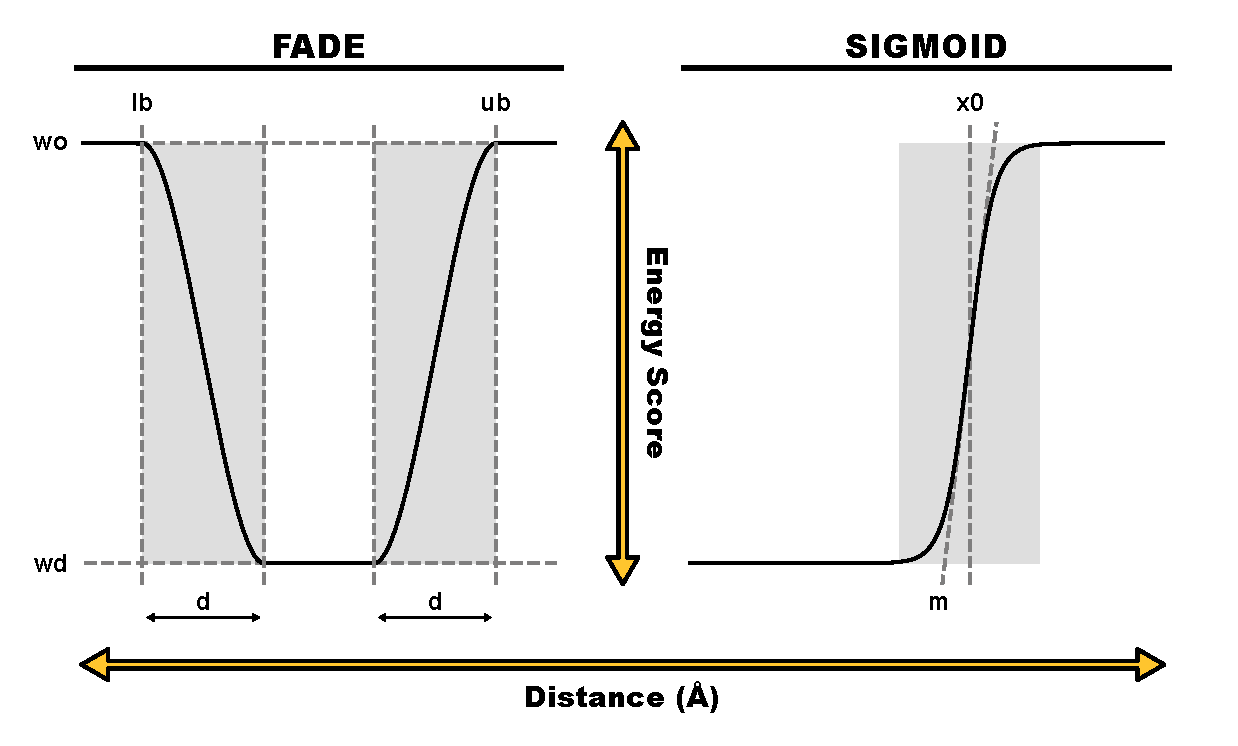
\includegraphics[width=\textwidth]{ample_predictors_efuncs.pdf}
    \caption{ROSETTA energy function comparison. Abbreviations corresponds to input parameters.}
    \label{fig:ample_predictors_efuncs}
\end{figure}

To explore the effects of the varying energy function definitions, we created six lists of contact restraints for each \textalpha-helical target and nine lists for each \textbeta-structure containing one. The top-ranking contact pairs per prediction were converted using the PCONSFOLD definition of the FADE function \cite{Michel2014-ci}, the GREMLIN definition of the SIGMOID function \cite{Ovchinnikov2015-nt}, and additionally the PCONSC2 BBCONTACTS definition of the FADE function for \textbeta-structure containing targets (see Chapter XYZ).

The conversion was handled in AMPLE (see Chapter XYZ) and invoked with the keywords outlined in table \ref{table:ample_predictors_kwargs}. The \texttt{-restraints\_factor} keyword defines the factor used to select contact pairs based on the target chain length, i.e. a factor of \texttt{1.5} would correspond to 3\textit{L}/2 contact pairs. The \texttt{-distance\_to\_neighbour} keyword defines the minimum distance in sequence space between contact pair participating residues, which were set to \texttt{5} residues for the FADE function \cite{Michel2014-ci} and \texttt{3} for the SIGMOID function \cite{Ovchinnikov2015-nt}. Additionally, all distance restraints were given an additional weight when introduced via the SIGMOID energy function to balance its energy term with all remaining terms in the ROSETTA scoring function (Sergey Ovchinnikov, personal communication). This was achieved by using the \texttt{-restraints\_weight} keyword and weights of \texttt{1.0} and \texttt{3.0} for the FADE and SIGMOID energy functions.

The addition of BBCONTACTS to existing sets of contacts was achieved with the FADE function in an identical manner as described in Chapter XYZ. In comparison, the SCALARWEIGHTED term in the GREMLIN implementation of the SIGMOID energy function \cite{Ovchinnikov2015-nt} was multiplied by the number of occurrences of each contact pair in the combined map.

\begin{table}[H]
    \centering
    \begin{tabularx}{\textwidth}{|X|X|}
        \hline
        \textbf{Energy Function} & \textbf{AMPLE keywords} \\
        \hline \hline
        \multirow{6}{1em}{FADE} & \texttt{-contact\_file <FILENAME>} \\
                                & \texttt{-contact\_format <FORMAT>} \\
                                & \texttt{-energy\_function FADE} \\
                                & \texttt{-restraints\_factor 1.0} \\
                                & \texttt{-distance\_to\_neighbour 5} \\
                                & \texttt{-restraints\_weight 1.0} \\
        \hline
        \multirow{6}{1em}{FADE (BBCONTACTS)} & \texttt{-contact\_file <FILENAME>} \\
                                & \texttt{-contact\_format <FORMAT>} \\
                                & \texttt{-energy\_function FADE} \\
                                & \texttt{-restraints\_factor 1.0} \\
                                & \texttt{-distance\_to\_neighbour 5} \\
                                & \texttt{-restraints\_weight 1.0} \\
        \hline
        \multirow{6}{1em}{SIGMOID} & \texttt{-contact\_file <FILENAME>} \\
                                & \texttt{-contact\_format <FORMAT>} \\
                                & \texttt{-energy\_function SIGMOID} \\
                                & \texttt{-restraints\_factor 1.5} \\
                                & \texttt{-distance\_to\_neighbour 3} \\
                                & \texttt{-restraints\_weight 3.0} \\
        \hline
        \multirow{6}{1em}{SIGMOID (BBCONTACTS)} & \texttt{-contact\_file <FILENAME>} \\
                                & \texttt{-contact\_format <FORMAT>} \\
                                & \texttt{-energy\_function SIGMOID\_bbcontacts} \\
                                & \texttt{-restraints\_factor 1.5} \\
                                & \texttt{-distance\_to\_neighbour 3} \\
                                & \texttt{-restraints\_weight 3.0} \\
        \hline
    \end{tabularx}
    \caption{Summary of AMPLE keyword arguments for FADE and SIGMOID ROSETTA energy functions.}
    \label{table:ample_predictors_kwargs}
\end{table}

\subsection{\textit{Ab initio} structure prediction}
Six or nine individual lists of contact restraints generated for each target were used in separate ROSETTA ab initio protein structure prediction runs. Additionally, protein structures were predicted without any contact restraints to acquire a control set of decoys. Homologous fragments were excluded during fragment library generation to imitate the folding process of a target with unknown fold. Fragment libraries were generated once per target and used throughout. In total, 1,000 ab initio decoys were generated per run using ROSETTA’s default settings \cite{Rohl2004-ou} and one of the seven contact conditions described previously. In total, 162 sets of models were generated across 18 protein targets.

\subsection{Molecular Replacement}
Besides considering model quality, one key interest of this study was the assessment of the model sets created in the previous step as ab initio Molecular Replacement search model templates. To reduce the enormous computational cost linked to trialling 162 sets of models, 108 sets were chosen from the following conditions: simple Rosetta, PCONSC2 prediction and FADE function, GREMLIN prediction and SIGMOID function, METAPSICOV prediction and FADE function, and where applicable, PCONSC2 BBCONTACTS, GREMLIN BBCONTACTS and METAPSICOV STAGE 1 BBCONTACTS predictions and FADE function. Overall, this resulted in four MR runs for the six \textalpha-helical targets, seven runs for the six all-\textbeta, and seven runs for the six mixed \textalpha-\textbeta\ targets. The resulting 108 model sets were trialled in AMPLE v1.1.0 and successful structure solution assessed (see Chapter XYZ).

\section{Results}
\subsection{Direct comparison of three contact metapredictors}
In this study, a direct comparison between three metapredictors - GREMLIN, METAPSICOV and PCONSC2 - was carried out. Residue-residue contact pairs were predicted for 18 protein target sequences with a range of chain lengths and numbers of effective sequences in their Pfam sequence alignments.

METAPSICOV is the most precise contact predictor across the protein target dataset in this study (Fig \ref{fig:ample_predictors_cutoff}). The difference between the three metapredictors is most evident in the highest-scoring contact pairs (\textit{L}/10). The median precision values for METAPSICOV and PCONSC2 contact predictions are above 50\% up to \textit{L} contact pairs. GREMLIN, in comparison, predicts contacts with a median precision score at least 20\% worse than that of METAPSICOV and 15\% worse than PCONSC2. However, at 3\textit{L}/2 contact pairs the median precision scores are much more similar across the three different metapredictors: METAPSICOV and PCONSC2 are near identical, and GREMLIN is at most 12\% worse compared to the other two. Inspecting the mean precision scores over a continuous range of selection cutoff values illustrates further the difference between METAPSICOV, PCONSC2 and GREMLIN (Fig \ref{fig:ample_predictors_covprc}). The former two similarly high precision scores compared to the average precision scores for GREMLIN, which are ~0.2 precision score units lower. Added to the difference in precision scores is the difference in sequence coverage (Fig \ref{fig:ample_predictors_covprc}). Although producing the on-average worst contact predictions out of the three metapredictors used in this study, GREMLIN contact predictions have the highest sequence coverage. However, an analysis of singleton contact pairs, usually with high degrees of false positives, revealed a positive correlation ($\rho_{Pearson}=0.47$; $p<0.001$) between the fraction of singleton contact pairs and sequence coverage and hints to a weak negative correlation ($\rho_{Pearson}=-0.27$; $p<0.05$) between the fraction of singleton contact pairs and contact precision (Fig \ref{fig:ample_predictors_singletons}).

\begin{figure}[H]
    \centering
    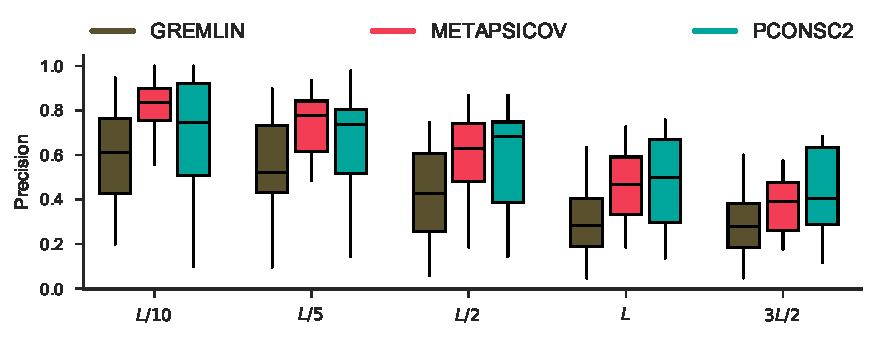
\includegraphics[width=\textwidth]{ample_predictors_cutoff.pdf}
    \caption{Precision spread for three metapredictors computed at five contact selection cutoff values relative to the target chain length (\textit{L}).}
    \label{fig:ample_predictors_cutoff}
\end{figure}

\begin{figure}[H]
    \centering
    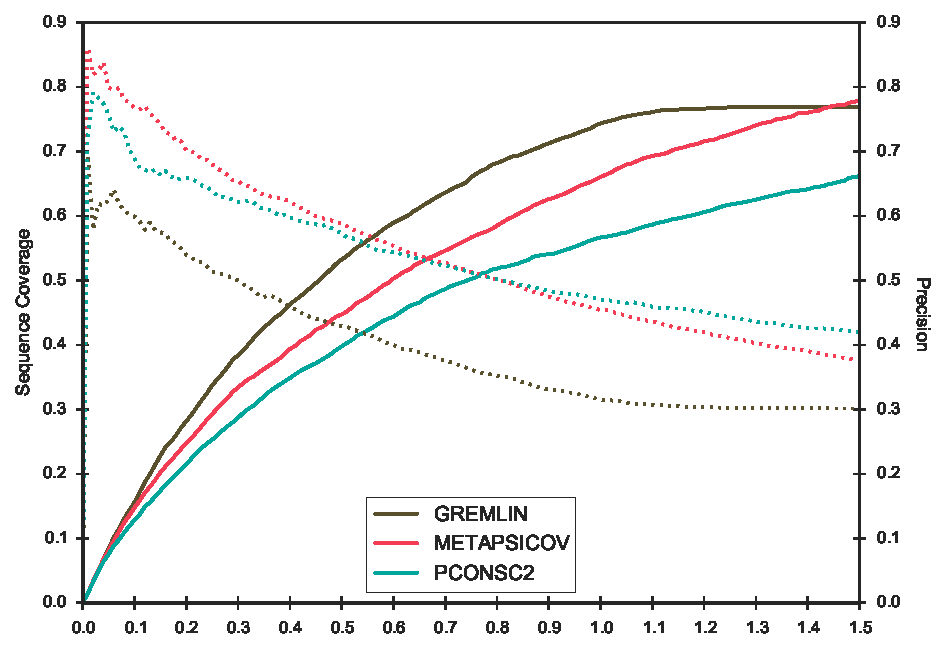
\includegraphics[width=\textwidth]{ample_predictors_covprc.pdf}
    \caption{Average sequence coverage (line) and contact prediction precision scores (dashed) across a continuous range of contact selection cutoffs ranging from $[0.0, 1.5]$ for all targets.}
    \label{fig:ample_predictors_covprc}
\end{figure}

\begin{figure}[H]
    \centering
    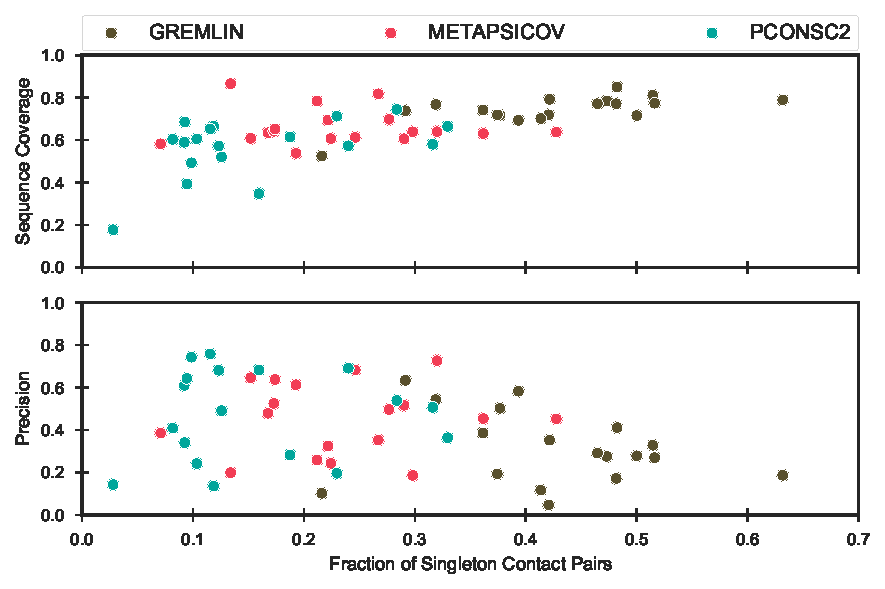
\includegraphics[width=\textwidth]{ample_predictors_singletons.pdf}
    \caption{Contact singleton analysis compared against the precision of \textit{L} contact pair lists for three metapredictors.}
    \label{fig:ample_predictors_singletons}
\end{figure}

Given that the overall precision of contact pairs predicted by the three metapredictors differs, it is important to understand where the difference originates. To investigate this, a comparison of the precision values at different cutoff levels on a per-target basis was performed. For the majority of targets the precision scores are very similar across the three metapredictors (Fig \ref{fig:ample_predictors_prcpeaks}). However, the prediction precision of some targets differs significantly. For example, the METAPSICOV prediction for the human retinoic acid nuclear receptor HRAR (PDB: 1fcy) contains high precision in its highest scoring (top-\textit{L}/10) contact pairs (Fig \ref{fig:ample_predictors_prcpeaks}). In comparison, GREMLIN and PCONSC2 predictions for the same target contain less precise contact pairs ($\Delta Precision_{METAPSICOV-GREMLIN} L/10=-0.522$; $\Delta Precision_{METAPSICOV-PCONSC2} L/10=-0.435$). However, the addition of further contact pairs up to 3\textit{L}/2 results in near-identical precision across the three metapredictors for this target. A second example illustrating such a difference are the contact predictions for the human galectin-3 CRD sequence (PDB: 4lbj). In contrast to the previous example, the data shows high precision scores for the METAPSICOV and PCONSC2 predictions for this target, yet low precision for the top GREMLIN contact pairs ($\Delta Precision_{METAPSICOV-GREMLIN} L/10=-0.231$; $\Delta Precision_{METAPSICOV-PCONSC2} L/10=+0.077$). 

\begin{figure}[H]
    \centering
    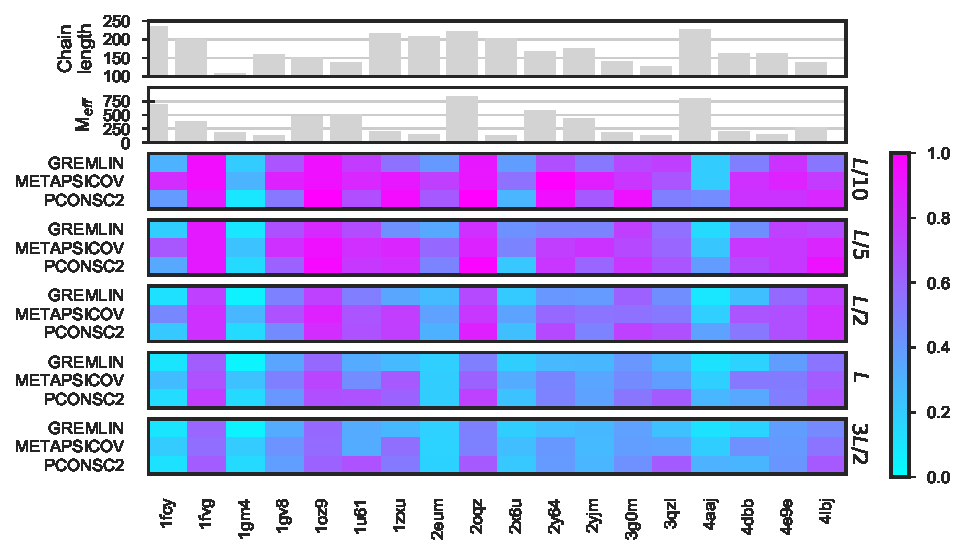
\includegraphics[width=\textwidth]{ample_predictors_prcpeaks.pdf}
    \caption{Contact prediction precision scores from three metapredictors for 18 targets at different contact pair selection thresholds. The Pfam alignment depth is given by means of number of effective sequences (\textit{Neff}). The color scale corresponds to the precision in $[0, 1]$.}
    \label{fig:ample_predictors_prcpeaks}
\end{figure}

The data presented in Fig \ref{fig:ample_predictors_prcpeaks} also indicates that there is no direct link between chain length or Neff and the precision of the resulting contact predictions. The N-(5'-phosphoribosyl)anthranilate isomerase sequence (PDB: 4aaj) with a chain length of 228 residues and 750 effective sequences in its Pfam alignment yielded a mean precision at \textit{L}/10 contact pairs of 0.283 (top-\textit{L}: 0.195) across the three metapredictors. This strongly contrasts with the sequence of sortase B (PDB: 2oqz), which shows similar characteristics yet obtained  mean precision at \textit{L}/10 contact pairs of 0.938 (top-\textit{L}: 0.622).

Although the contact predictions differ in precision, an interesting question rests with the similarity of the predicted contact pairs amongst the sets. Thus, the similarity of contact predictions across the three metapredictors is an important metric to evaluate the most appropriate algorithm for AMPLE users. Using the Jaccard similarity index to evaluate the direct overlap of contact pairs across sets of predictions, the data suggests very little similarity between the contact predictions of the three metapredictors for each target (Fig \ref{fig:ample_predictors_jaccardidx}). As with the differences in precision scores at higher cutoff thresholds, the Jaccard index is also lower - indicating less overlap - at higher cutoff thresholds. However, it is worth noting that the Jaccard index only considers identical matches and does not consider the neighbourhood of a contact pair. Thus, the index does not highlight similar regions with contact pairs in both maps.

\begin{figure}[H]
    \centering
    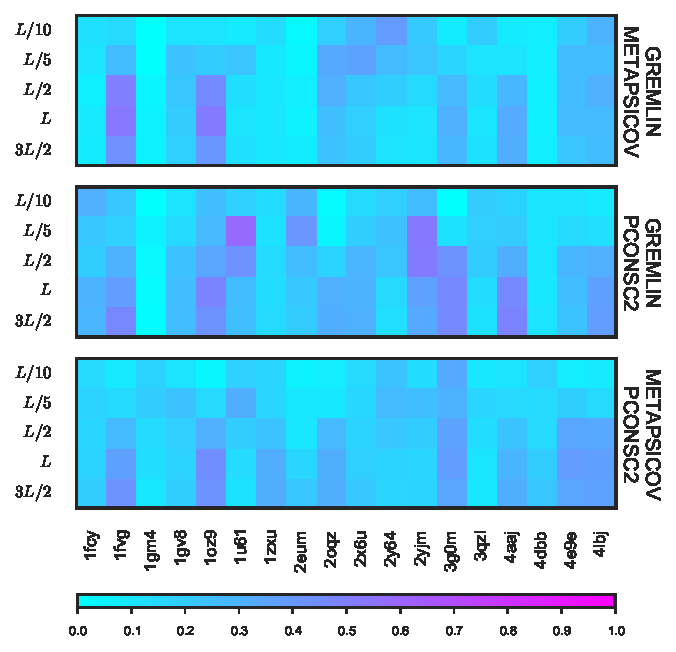
\includegraphics[width=\textwidth]{ample_predictors_jaccardidx.pdf}
    \caption{Jaccard similarity index illustrates a higher degree of overlap between metapredictor contact predictions with increasing numbers of contact pairs included in the calculation. The three panels show the different comparisons. The color scale corresponds to the Jaccard index in $[0, 1]$.}
    \label{fig:ample_predictors_jaccardidx}
\end{figure}

\subsection{Protein structure prediction with two ROSETTA energy functions}
The accuracy of the starting decoys is a major factor for an AMPLE run to succeed \cite{Simkovic2016-jx, Thomas2017-lq}. Thus, the quality of the decoys is of great essence to this study. Given the two different ROSETTA energy functions, FADE and SIGMOID, all contacts predicted were subjected to individual ab initio structure prediction runs. Additionally, all contact predictions were enriched with BBCONTACTS for all \textbeta-containing targets in separate trials. A total of 234,000 individual decoys were generated in this study through all permutations of targets, contact predictions and ROSETTA energy function combinations.

Separating these individual decoys solely by the ROSETTA energy function (excluding unrestrained ROSETTA decoys) shows that the FADE energy function results in marginally more accurate decoys (median TM-score FADE: 0.3541; median TM-score SIGMOID: 0.2969). To further investigate which energy function is more suitable for the target dataset used in this study, the decoy sets were grouped by two additional characteristics: the fold of the target, and the source of distance restraints used. The results strongly suggest that the FADE energy function results in more accurate decoy sets (Fig \ref{fig:ample_predictor_tmmedian}), outperforming the SIGMOID energy function by median TM-score in two-thirds of all decoys sets (FADE: 58; SIGMOID: 32). A split of the decoy sets into separate categories by fold and the addition of BBCONTACTS reveals that the SIGMOID energy function only yields similar results for all-\textbeta\ targets in combination with BBCONTACTS-supported distance restraints. Although the total count of decoy sets with higher accuracies between the two energy functions in this category are similar, the actual differences in TM-scores further supports the strength of the FADE energy function compared to the SIGMOID.

\begin{figure}[H]
    \centering
    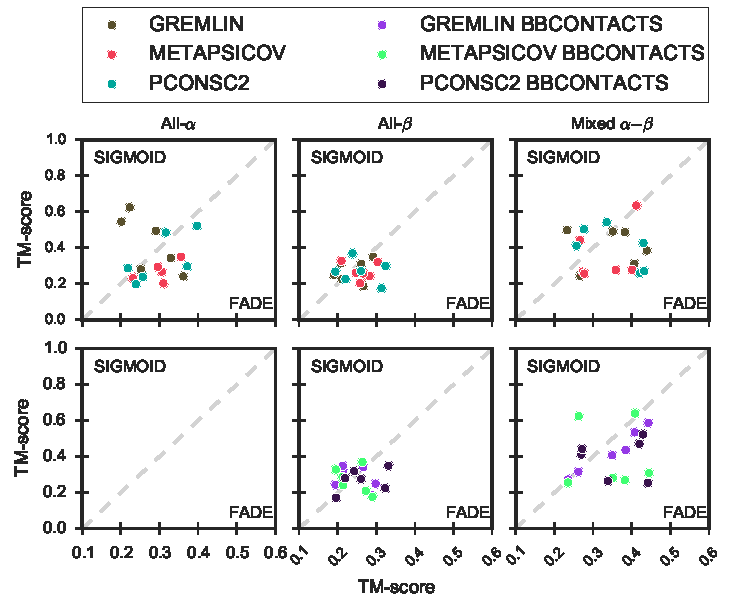
\includegraphics[width=\textwidth]{ample_predictors_tmmedian.pdf}
    \caption{Median TM-score comparison of FADE and SIGMOID ROSETTA energy functions differentiated by fold and the addition of BBCONTACTS restraints.}
    \label{fig:ample_predictor_tmmedian}
\end{figure}

Besides the structure prediction accuracy of each set of decoys, the single, most accurate decoy is also of great interest. If one energy function consistently predicts single decoys more accurately, it might be appropriate to reconsider the structure identification routine (i.e. clustering) in AMPLE for search model preparation. However, a similar difference to that of the decoy quality of entire sets is observed for the top-1 decoy in each set (Fig \ref{fig:ample_predictor_tmtop}). The FADE energy function outperforms the SIGMOID function for the majority of target-contact prediction permutations (FADE: 51; SIGMOID: 39). However, the GREMLIN distance restraints in combination with the SIGMOID energy function produce better top-1 decoys than GREMLIN restraints with the FADE energy function. This suggests that GREMLIN restraints and the SIGMOID energy function were tailored to complement each other with the ultimate goal of predicting single decoys to high accuracy over entire sets of decoys. Additionally, the spread of decoy quality differences between the two energy functions widens when only looking at the best decoy in each predicted set ($\Delta Median TM-score_{ALL}: min=0.002, max=0.429$; $\Delta Median TM-score_{TOP}: min=0.002, max=0.456$). 

\begin{figure}[H]
    \centering
    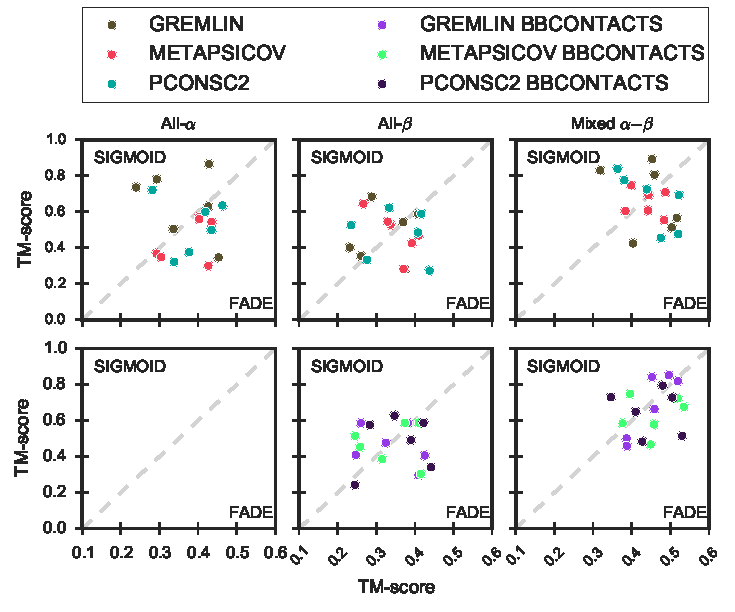
\includegraphics[width=\textwidth]{ample_predictors_tmtop.pdf}
    \caption{Top TM-score comparison of FADE and SIGMOID ROSETTA energy functions differentiated by fold and the addition of BBCONTACTS restraints.}
    \label{fig:ample_predictor_tmtop}
\end{figure}

A \acrfull{kde} of TM-scores using each predicted decoy was generated with the TM-scores of individual decoys separated only by fold class and ROSETTA energy function (Fig \ref{fig:ample_predictor_tmdensity}). This density estimate further supports the results presented above: the FADE energy function generates more accurate decoys. However, a very important detail is highlighted by the estimates. Distinct regions with high density are visible in the estimates of the TM-scores of individual decoys for all-\textalpha\ and mixed \textalpha-\textbeta\ targets (Fig \ref{fig:ample_predictor_tmdensity}). The bimodal distribution of decoy TM-scores from both energy functions strongly suggests that predicted structures are either native-like or not (based on the TM-score threshold of $\leq0.5$). However, the number of correctly predicted decoys versus incorrectly predicted decoys is in favour of the latter. The decoy sets of all-\textbeta\ targets do not show such distinct regions of high density for decoys with TM-scores $<0.5$ units in any of its density estimates (Fig \ref{fig:ample_predictor_tmdensity}). The generally poor decoy quality of decoys predicted without any distance restraint information (ROSETTA) highlights the benefit of contact predictions to ab initio protein structure prediction.

\begin{figure}[H]
    \centering
    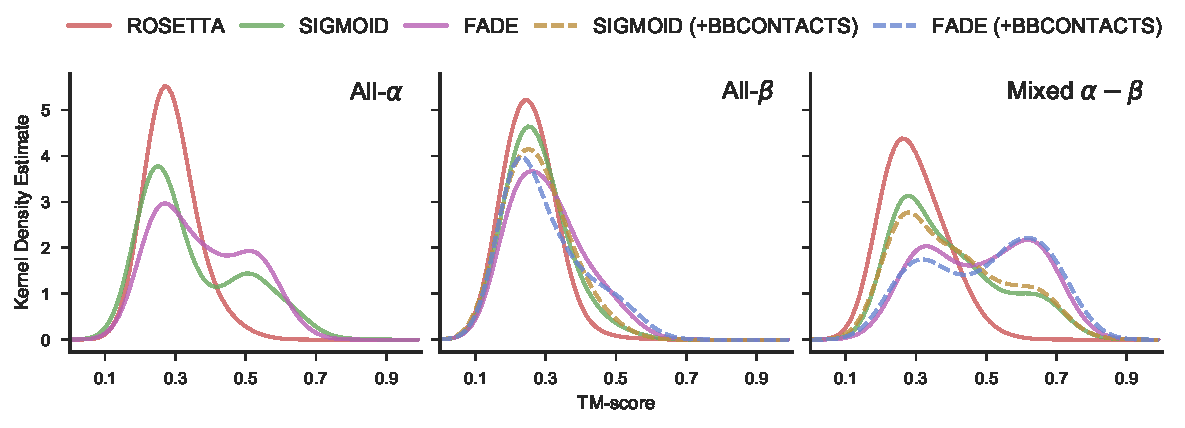
\includegraphics[width=\textwidth]{ample_predictors_tmdensity.pdf}
    \caption{TM-score density estimate of all decoys in each respective fold class separating by ROSETTA energy function (SIGMOID or FADE) and no contact information used (ROSETTA). Dashed lines indicate decoys which were predicted with the addition of BBCONTACTS.}
    \label{fig:ample_predictor_tmdensity}
\end{figure}

A further important aspect of this study is to explore the benefits of adding BBCONTACTS restraints to the structure prediction of \textbeta-containing targets. Although previous results (see Chapter XYZ) in combination with those presented above outline overall improvements in decoy quality, it is essential to understand which targets benefit from this treatment. Figure \ref{fig:ample_predictor_bbdir} highlights the effects of adding BBCONTACTS restraints to the structure prediction strategies employed here. In summary, the addition of BBCONTACTS restraints hardly affects the decoy quality of most targets under the various contact prediction and energy function combinations. Nevertheless, three target, contact prediction and energy function combinations yielded TM-score improvements of at least 0.1 TM-score units compared to the same condition without the addition of BBCONTACTS restraints. In contrast, the addition of BBCONTACTS restraints did not lower the median TM-score by more than 0.1 units for any target (Fig \ref{fig:ample_predictor_bbdif}).

\begin{figure}[H]
    \centering

    \begin{subfigure}[b]{\textwidth}
        \centering
        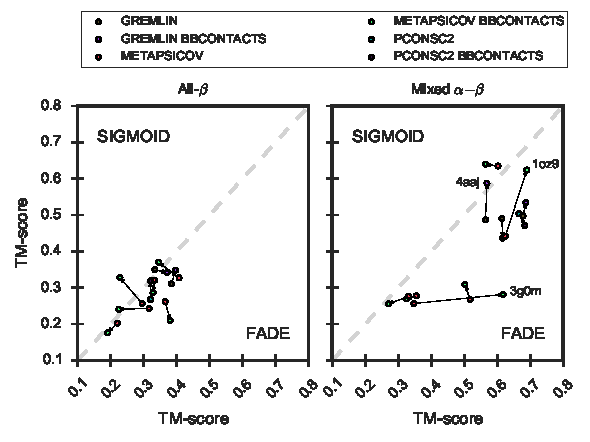
\includegraphics[width=0.9\textwidth]{ample_predictors_bbdir.pdf}
        \caption{}
        \label{fig:ample_predictor_bbdir}
    \end{subfigure}
    
    \begin{subfigure}[b]{\textwidth}
        \centering
        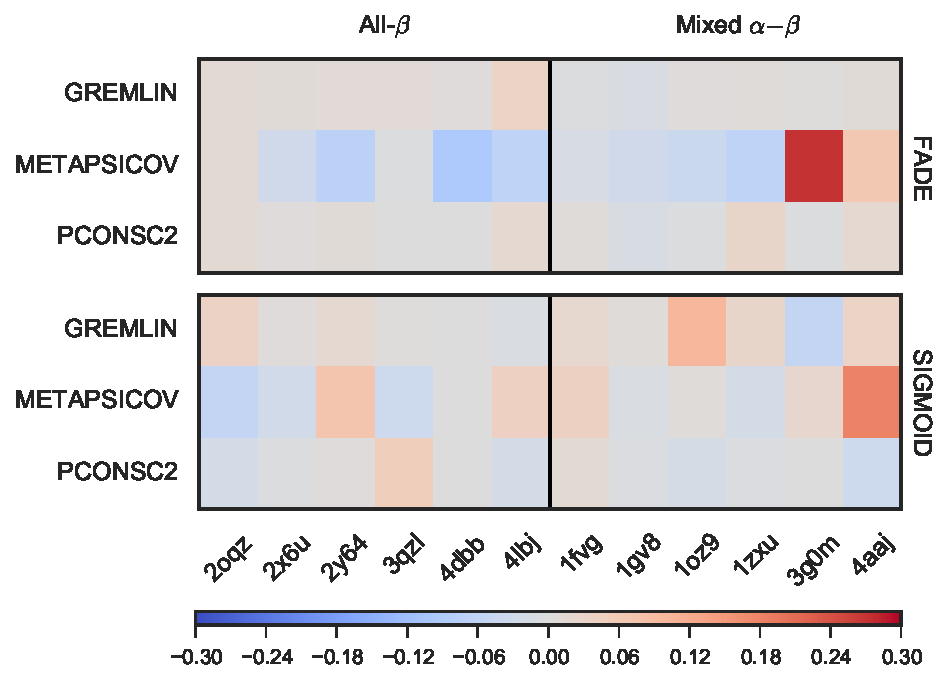
\includegraphics[width=0.9\textwidth]{ample_predictors_bbdif.pdf}
        \caption{}
        \label{fig:ample_predictor_bbdif}
    \end{subfigure}

    \caption{Median TM-score comparison of FADE and SIGMOID ROSETTA energy functions differentiated by fold (excl. all-\textalpha). (a) Arrows indicate the effect on decoy quality through the addition of BBCONTACTS restraints. Targets with a distance $<0.03$ TM-score units between normal and BBCONTACTS-added conditions were excluded from the scatter plots. (b) Effect on decoy quality through the addition of BBCONTACTS restraints highlighted by heatmap difference. The color scale corresponds to the difference in median TM-score between normal and BBCONTACTS-added contact maps.}
\end{figure}

Two further aspects in understanding the differences in effects of the FADE and SIGMOID ROSETTA energy functions on decoy quality are the target chain length and restraints precision. The former appears to affect the final decoy quality of all 1,000 decoys insignificantly (Fig \ref{fig:ample_predictor_tmsummary}). However, the restraint precision results in some differences between the two ROSETTA energy functions (Fig \ref{fig:ample_predictor_tmsummary}). The FADE energy function (L restraints) generally appears to be less sensitive to restraint lists with higher false positive contact pairs.  In contrast, the SIGMOID function  (3\textit{L}/2 restraints) produces less accurate decoys than the FADE function with more accurate restraints. Most strikingly, the FADE energy function generated decoys with a median TM-score of 0.678 for the N-(5'-phosphoribosyl)anthranilate isomerase domain (PDB: 4aaj) compared to the SIGMOID function with a median TM-score of 0.498. Nevertheless, both energy functions appear to broadly follow a positive linear trend, i.e. better restraint precision results in more accurate decoys.

\begin{figure}[H]
    \centering
    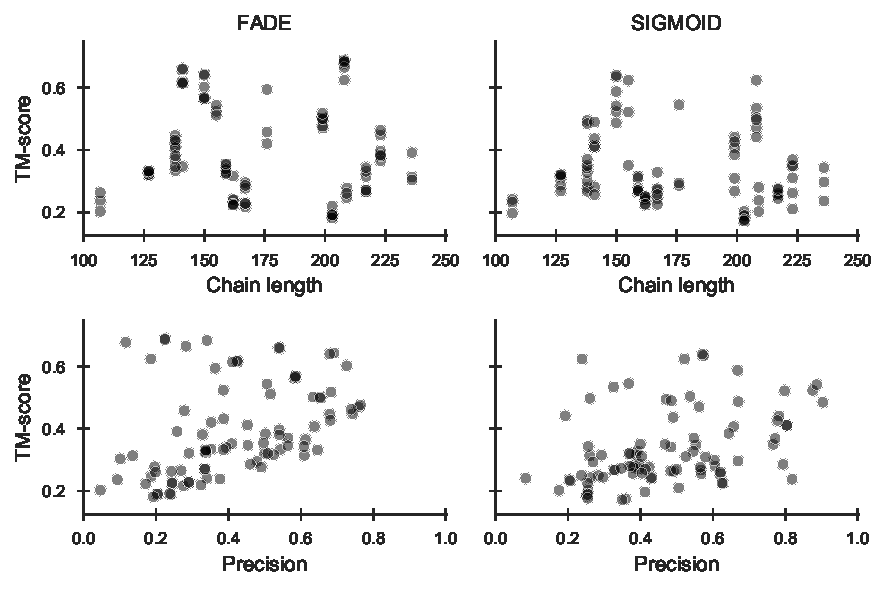
\includegraphics[width=\textwidth]{ample_predictors_tmsummary.pdf}
    \caption{Effects of target chain length and restraint precision on the median TM-score for FADE and SIGMOID ROSETTA energy functions. Each scatter point represents a 1,000-decoy set.}
    \label{fig:ample_predictor_tmsummary}
\end{figure}

\subsection{Impact of metapredictors and energy functions on unconventional MR}
The results obtained from the decoy quality comparison outlined above highlighted differences between the FADE and SIGMOID ROSETTA energy functions. This difference is more pronounced for some targets and less so for others. Thus, the next step in this study was to analyse the consequences  of these differences for unconventional MR using the automated pipeline AMPLE.

Overall, the decoys restrained with GREMLIN distance restraints via the SIGMOID energy function throughout the structure prediction process yielded six out of 18 possible structure solutions (Fig \ref{fig:ample_predictor_ample}). This result was the highest of all trialled conditions and only resulted in one more structure solution compared to unrestrained ROSETTA decoys. Surprisingly, all remaining conditions resulted in fewer structure solutions than those from ROSETTA decoys. Furthermore, the conditions METAPSICOV (FADE function), METAPSICOV BBCONTACTS (FADE function) and PCONSC2 BBCONTACTS (FADE function) yielded no more than half of the structure solutions achieved by GREMLIN (SIGMOID function). The remaining two conditions - PCONSC2 (FADE function) and GREMLIN BBCONTACTS (FADE function) - resulted in four out of 18 structure solutions. The addition of BBCONTACTS did not improve decoy quality enough to increase the chances of structure solution success; however, the structure of the bovine peptide methionine sulfoxide reductase (PDB: 1fvg) was only solved with the GREMLIN BBCONTACTS (FADE function) decoys further supporting the small but important value of BBCONTACTS restraint addition to separately determined contact predictions (see Chapter XYZ).

\begin{figure}[H]
    \centering
    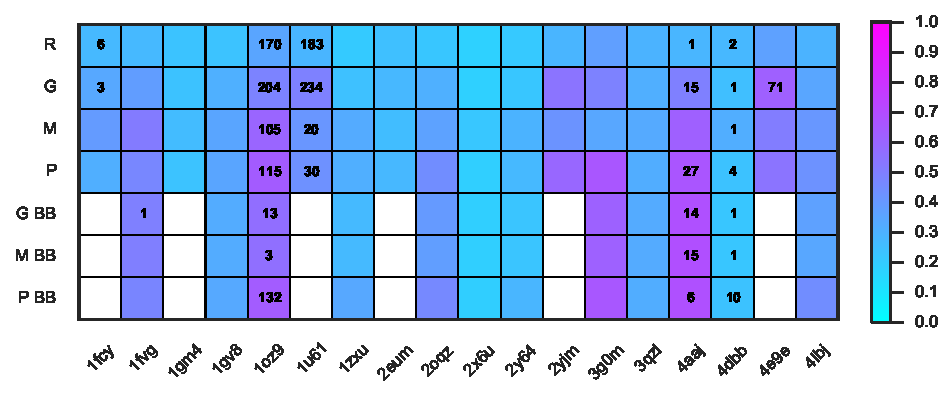
\includegraphics[width=\textwidth]{ample_predictors_ample.pdf}
    \caption{Structure solution count for AMPLE search models generated from decoys with varying contact prediction and ROSETTA energy function conditions: unrestrained ROSETTA (R); GREMLIN (G; SIGMOID function); METAPSICOV (M; FADE function); PCONSC2  (P; FADE function); GREMLIN BBCONTACTS (G BB; FADE function); METAPSICOV BBCONTACTS (M BB; FADE function); PCONSC2 BBCONTACTS (P BB; FADE function). The color scale of each square indicates the median TM-score of all 1,000 starting decoys.}
    \label{fig:ample_predictor_ample}
\end{figure}

The number of structure solutions obtained from the decoy sets subjected to the AMPLE pipeline are somewhat surprising given that ROSETTA decoys result in the second-most structure solutions. These results suggest that the current implementation cannot exploit the true value of more accurate decoy sets. This hypothesis is further supported when considering the decoy set quality and the number of structure solutions (Fig \ref{fig:ample_predictor_ample}). For example, PCONSC2 (FADE function) decoys predicted for the hypothetical protein AQ\_1354 (PDB: 1oz9) yield high accuracy, and thus would generally be considered highly desirable starting structures for the AMPLE protocol; nevertheless, the AMPLE protocol was unable to exploit such highly accurate decoys for successful structure solutions of other targets, e.g. cysteine desulferation protein SufE (PDB: 3g0m; $median TM-score PCONSC2 BBCONTACTS (FADE function)=0.661$). In comparison, the median TM-scores for all successful ROSETTA decoy sets do not exceed 0.355 TM-score units.

Naturally, one would expect the best decoys to result in the most accurate ensemble search models, which in turn yield the highest number of structure solutions per target. However, here we demonstrate that the most accurate decoys do not guarantee structure solution, and in contrast some poorly predicted decoy sets achieve structure solution. Thus, it is essential to investigate the stage in AMPLE’s cluster-and-truncate approach at which the higher decoy quality results in less suitable ensemble search models for MR.

The data generated as part of this study reveals a positive correlation ($\rho_{Spearman}=0.78$; $p<0.001$) between the decoy quality and the number of resulting AMPLE ensemble search models (Fig \ref{fig:ample_predictor_ensdep}). The plotted data alongside a fitted LOWESS function further illustrate that small differences in decoy quality in the lower TM-score regions increases the total number of generated ensemble search models dramatically. However, once the threshold of 0.5 TM-score units \cite{Xu2010-sw} is surpassed the number of generated ensemble search models plateaus at around ~350-400 ensemble search models, approaching the maximum number of search models generatable by AMPLE. Furthermore, the data suggests that sets containing fewer than 100 ensemble search models do not lead to structure solution, although this result needs to be considered with care given the difficulty of predicting which search model will lead to structure solution.

\begin{figure}[H]
    \centering
    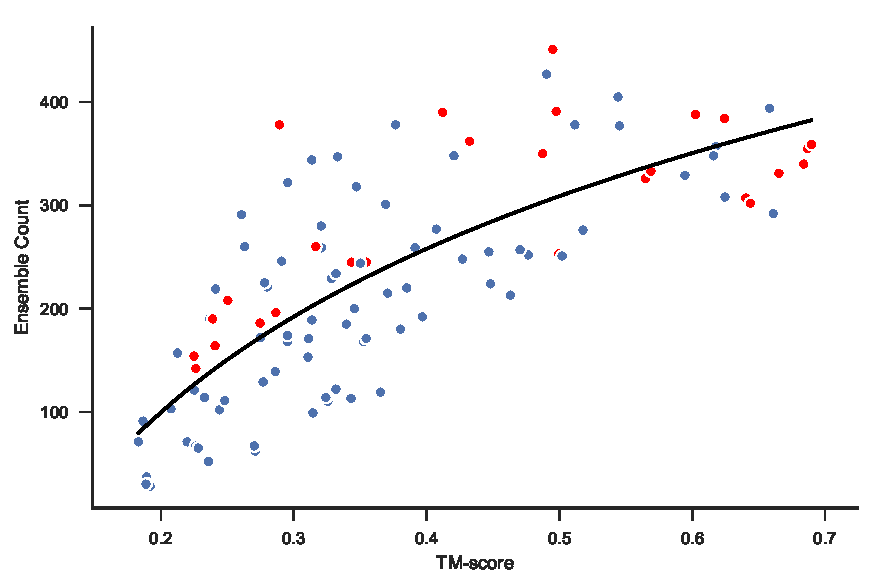
\includegraphics[width=\textwidth]{ample_predictors_ensdep.pdf}
    \caption{Comparison of median TM-score comparison (per 1,000 decoys) against the resulting AMPLE ensemble search model count. LOWESS function fitted to data to illustrate relationship. Red dots indicate successful ensemble sets.}
    \label{fig:ample_predictor_ensdep}
\end{figure}

Besides looking at the relationship between entire decoy sets and the resulting structure solutions on a per-target or per-condition basis, it is important to also consider individual ensemble search models, their origins and their properties in relation to MR metrics. Previous findings highlighted the relationship between the number of decoys in the first cluster and the quality of the decoys it contains (see Chapter XYZ). Here, we further support these findings given the positive relationship between the median TM-scores and the corresponding size of the largest SPICKER cluster (Fig \ref{fig:ample_predictor_clusizetm}). An analysis of the cluster sizes demonstrates the downstream benefits of increased decoy quality through contact restraints in the folding process (Fig \ref{fig:ample_predictor_clusize}). The sizes of the first three clusters generated from most contact-restraint decoy sets greatly surpass their equivalent cluster sizes for unrestrained ROSETTA decoys. Given that cluster sizes correlate with decoy quality, the findings in this study also support that the mean C\textalpha\ R.M.S.D. - as calculated by THESEUS for cluster truncation - is directly related to better decoy quality via the larger number of decoys in each cluster (Fig \ref{fig:ample_predictor_clurmsd}). The same mean C\textalpha\ R.M.S.D. is also related to the number of ensemble search models generated after subclustering (Fig \ref{fig:ample_predictor_rmsdsm}), which hints towards a direct relationship between increased quality of 1,000 decoys per set and the total number of ensemble search models generated. Interestingly, GREMLIN decoys show similar C\textalpha\ R.M.S.D. per cluster compared to unrestrained ROSETTA decoys (Fig \ref{fig:ample_predictor_carmsd}), unlike all other contact restraint guided structure predictions. However, it is worth noting that almost no distinction can be made amongst the remaining contact restraint treatments albeit some differences in cluster size distributions exist (Fig \ref{fig:ample_predictor_clusize}).

\begin{figure}[H]
    \centering
    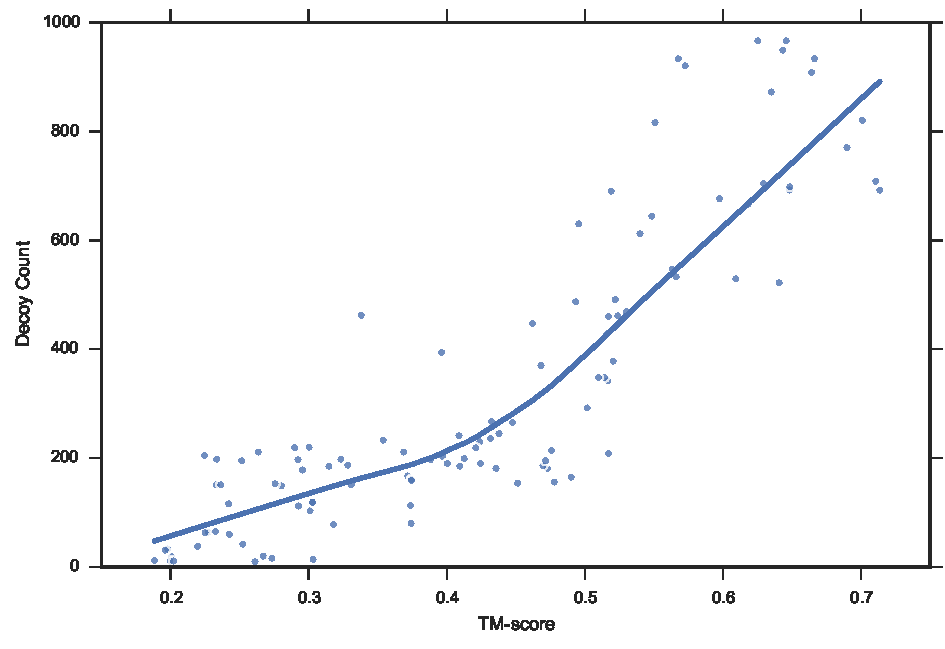
\includegraphics[width=\textwidth]{ample_predictors_clusizetm.pdf}
    \caption{Relationship between cluster median TM-score and the number of cluster decoys. Blue line represents LOWESS relationship fitted to data.}
    \label{fig:ample_predictor_clusizetm}
\end{figure}

\begin{figure}[H]
    \centering
    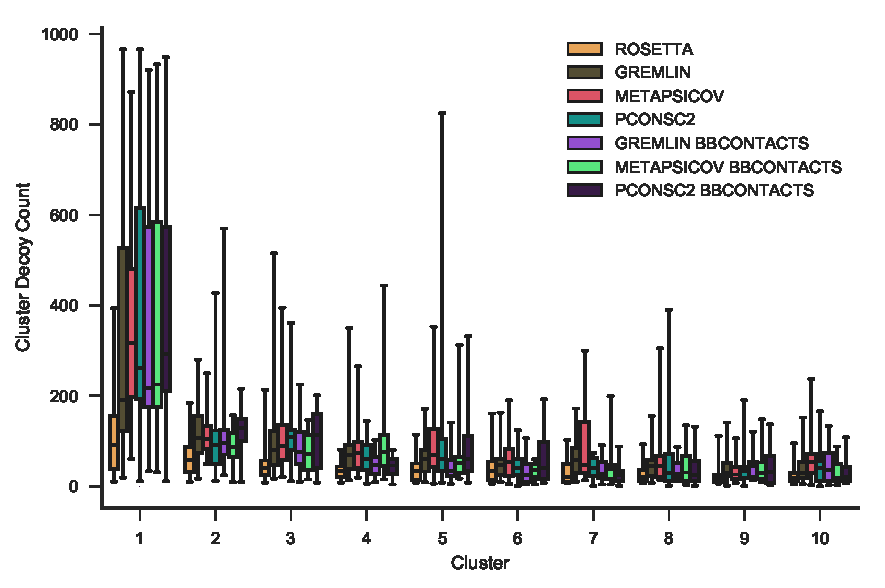
\includegraphics[width=\textwidth]{ample_predictors_clusize.pdf}
    \caption{SPICKER cluster sizes of each target grouped the restraint condition used during the structure prediction protocol. Whiskers span the range from the minimum to maximum counts.}
    \label{fig:ample_predictor_clusize}
\end{figure}

\begin{figure}[H]
    \centering
    \begin{subfigure}[b]{\textwidth}
        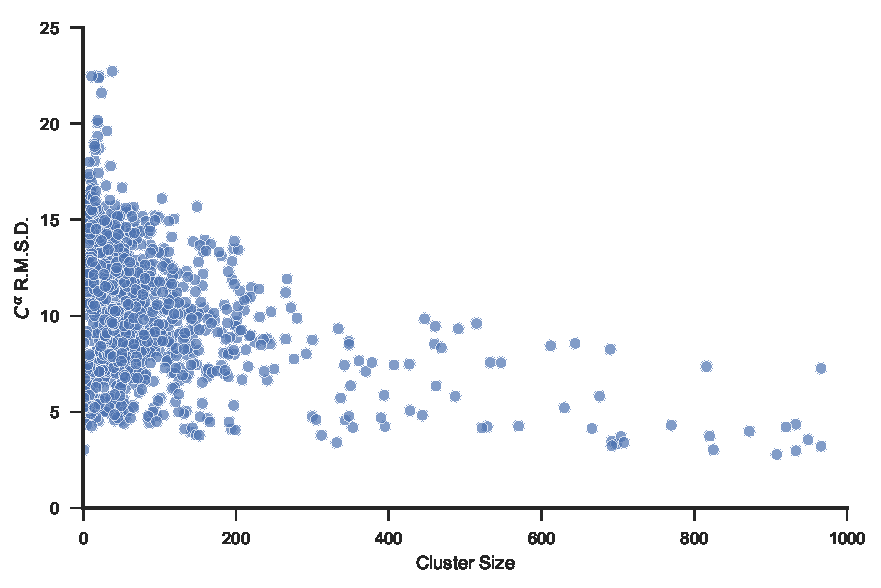
\includegraphics[width=\textwidth]{ample_predictors_clurmsd.pdf}
        \caption{}
        \label{fig:ample_predictor_clurmsd}
    \end{subfigure}
    \begin{subfigure}[b]{\textwidth}
        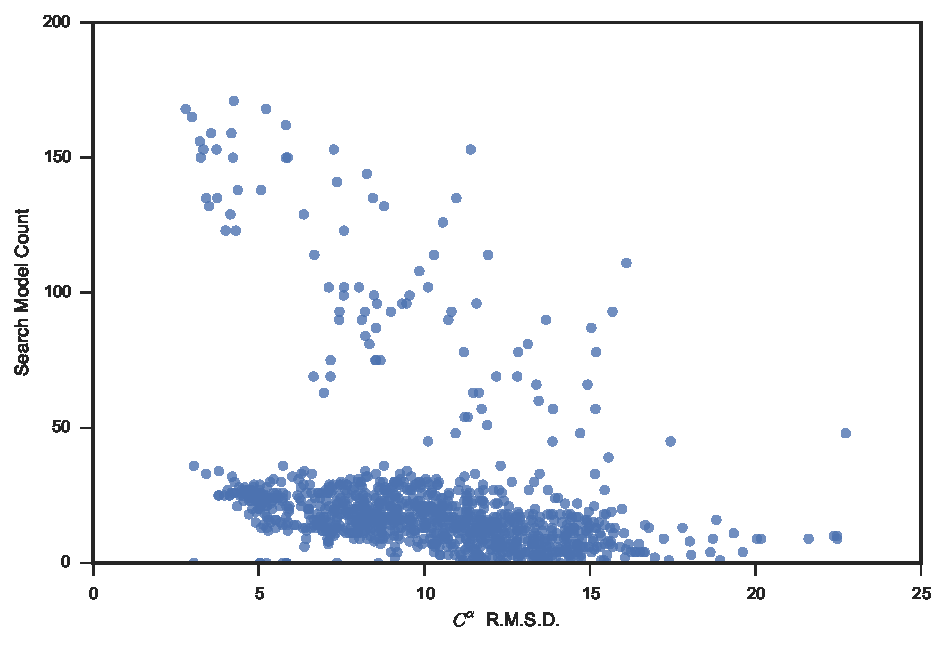
\includegraphics[width=\textwidth]{ample_predictors_rmsdsm.pdf}
        \caption{}
        \label{fig:ample_predictor_rmsdsm}
    \end{subfigure}

    \caption{(a) Number of decoys per SPICKER cluster plotted against the mean C\textalpha-atom R.M.S.D. for all decoys in each cluster. (b) Mean C\textalpha-atom R.M.S.D. for decoys per cluster plotted against the number of search models derived from the cluster.}
\end{figure}


\begin{figure}[H]
    \centering
    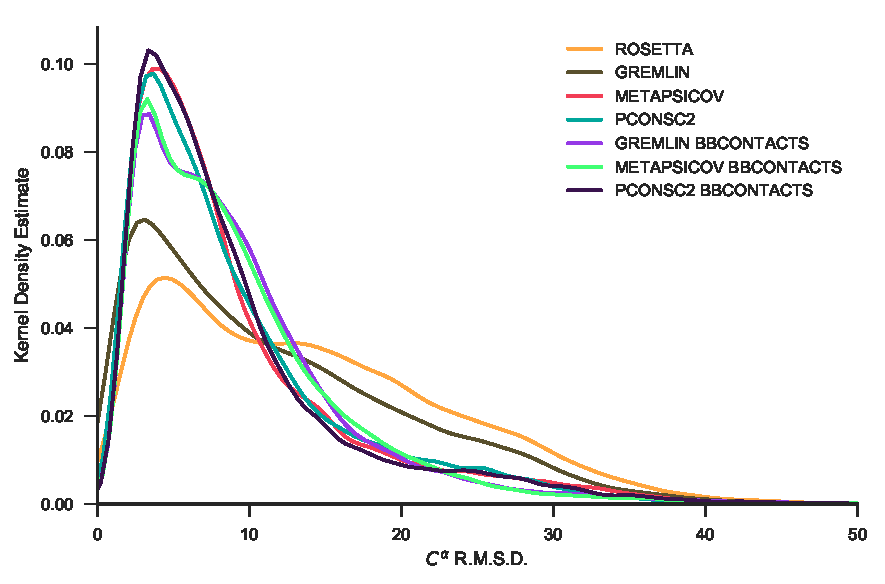
\includegraphics[width=\textwidth]{ample_predictors_carmsd.pdf}
    \caption{Kernel density estimate of C\textalpha\ interatomic R.M.S.D. for SPICKER clusters.}
    \label{fig:ample_predictor_carmsd}
\end{figure}


The structure solution through pipelines like AMPLE and other unconventional MR software \cite{Rodriguez2009-tk, Sammito2013-tt} can result from the placement of generated (ensemble) search models either in- or out-of-sequence register. The RIO metric \cite{Thomas2015-ag} can reliably assess the register placement, and thus was used to analyse the MR placements of all search models of the seven targets with structure solutions from one or more decoy sets. The RIO scores for the hypothetical protein AQ\_1354 (PDB: 1oz9) strongly support the high quality decoys used as input across all seven contact conditions (Fig \ref{fig:ample_predictor_riotar}). Most search models are placed in-register and hardly any search models with out-of-register RIO scores failed either. In contrast, the search models of N-(5’-phosphoribosyl)anthranilate isomerase (PDB: 4aaj) - derived from high quality decoys in most conditions - shows a low percentage of AMPLE search models with RIO scores leading to structure solution (Fig \ref{fig:ample_predictor_riotar}). Furthermore, the RIO scores normalized by the target chain length indicate that search models, independent of MR structure solution, were relatively small only exceeding 20\% of the total target sequence in a few cases. 

\begin{figure}[H]
    \centering
    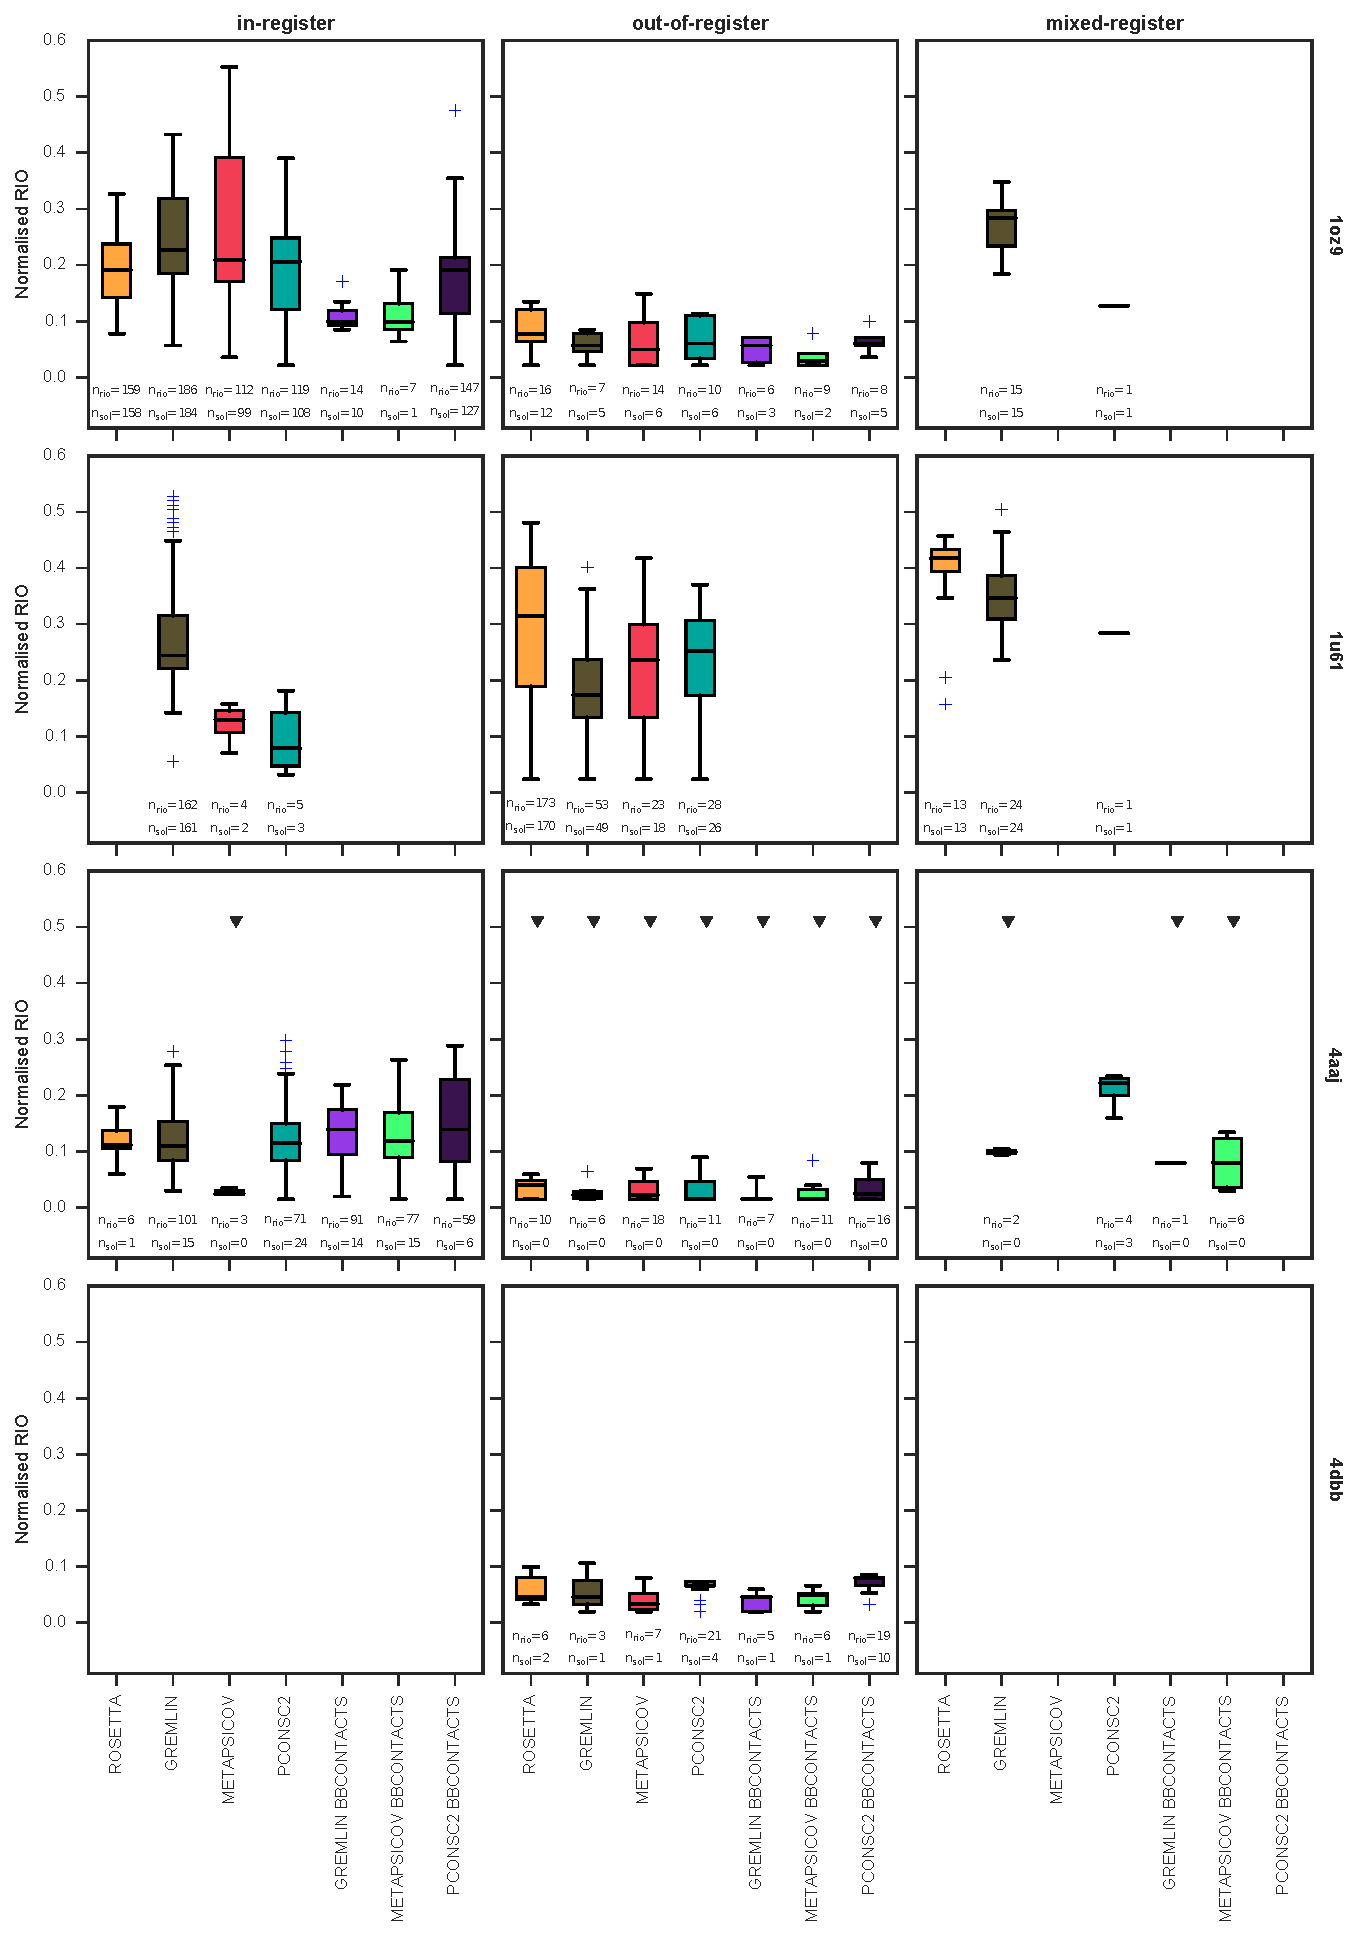
\includegraphics[width=\textwidth]{ample_predictors_riotar.pdf}
    \caption{Normalised RIO score analysis of four successful targets in the MR dataset. Black triangles indicate AMPLE search model sets without a structure solution.}
    \label{fig:ample_predictor_riotar}
\end{figure}

One interesting target in this set with respect to the sequence register of the AMPLE search models leading to structure solution is putative ribonuclease III (PDB: 1u61). Although decoys from all contact conditions readily solved this target with at least 20 or more AMPLE search models, one interesting aspect arises from the RIO register analysis. Only GREMLIN decoys are primarily placed in-register (Fig \ref{fig:ample_predictor_riotar}). AMPLE search models derived from the other three contact conditions, and in particular those from ROSETTA decoys, are primarily placed out-of-register with sequence coverage values of roughly 25\%. In fact, a close analysis of the diversity of AMPLE search models highlights the accuracy of GREMLIN search models which represent a closely-matched substructure of the target protein (Fig \ref{fig:ample_predictors_1u61_c2_t70_r1_reliable}).  

\begin{figure}[H]
    \centering
    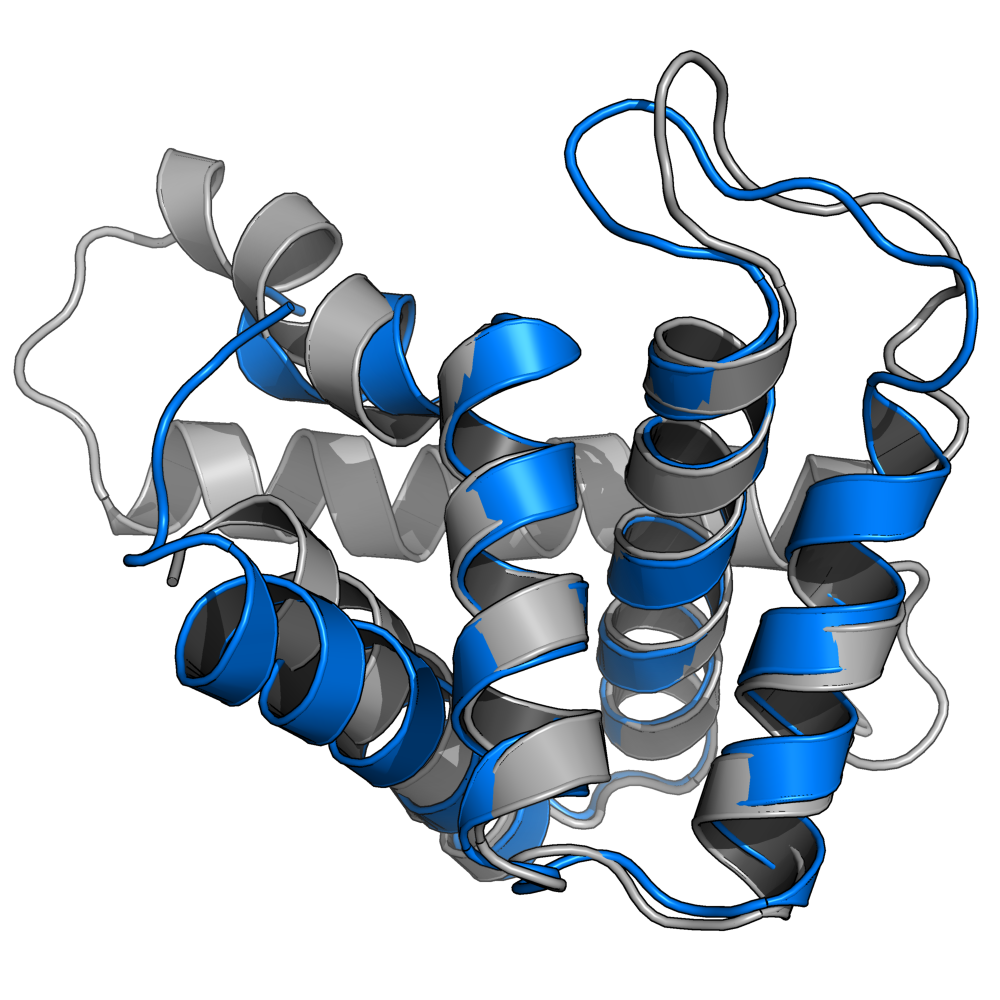
\includegraphics[width=\textwidth]{ample_predictors_1u61_c2_t70_r1_reliable.png}
    \caption{Successful search model (blue cartoon) post-PHASER placement superposed with the native structure (gray cartoon) for putative ribonuclease III (PDB: 1u61).}
    \label{fig:ample_predictors_1u61_c2_t70_r1_reliable}
\end{figure}

Compared to all other targets with structure solutions in at least one condition, the PTB domain of Mint1 (PDB: 4dbb) produced interesting yet somewhat surprising results. None of the search models, independent of their decoy source, achieved correct placement with any residue being in register. All structure solutions were obtained from out-of-register search model placements (Fig \ref{fig:ample_predictor_riotar}). A visual inspection of all successful search models revealed that structure solutions were exclusively obtained with idealised fragments. ROSETTA, GREMLIN and METAPSICOV decoys resulted in one or more single-helix ensemble search models that led to structure solution (Fig \ref{fig:ample_predictors_4dbb_esm_egs}). More interestingly though, PCONSC2, GREMLIN BBCONTACTS, METAPSICOV BBCONTACTS and PCONSC2 BBCONTACTS decoys yielded one or more two-strand \textbeta-sheets which, after successful MR, yielded fully built structures (Fig \ref{fig:ample_predictors_4dbb_esm_egs}).

\begin{figure}[H]
    \centering
    \includegraphics[width=\textwidth]{ample_predictors_4dbb_esm_egs.png}
    \caption{Successful search models post-PHASER placement (blue) superposed to the reference crystal structure (grey) for PTB domain of Mint1 (PDB: 4dbb).}
    \label{fig:ample_predictors_4dbb_esm_egs}
\end{figure}

Lastly, three targets were solved with one or two decoy sets alone. The structures of the retinoic acid nuclear receptor HRAR (PDB: 1fcy) and the peptide methionine sulfoxide reductase (PDB: 1fvg) were only solved with a handful of AMPLE search models. Often singleton solutions like these are achieved through AMPLE’s cluster-and-truncate procedure producing a single, idealised helix as search model. Here, we confirm such findings for target 1fcy, whereby single out-of-register helices derived from ROSETTA and GREMLIN decoys achieved structure solutions. However, the singleton search model derived from the GREMLIN BBCONTACTS decoys for the peptide methionine sulfoxide reductase (PDB: 1fvg) was placed in-register. A closer inspection of this AMPLE ensemble search model highlights a great success of the approach of adding BBCONTACTS distance restraints to separately predicted contact maps. In this instance, the successful AMPLE ensemble search model has 77\% of its 49 residues placed in-register. More importantly, the search model is made up of two \textbeta-strands packing against each other, which was supported by BBCONTACTS predictions (Fig \ref{fig:ample_predictors_1fvg_gbb_phaser_c1_t25_r3_polyAla}). The last case, glycosylase domain of MBD4 (PDB: 4e9e), solved solely with GREMLIN decoys yielding 71 structure solutions. All successful AMPLE search models derived from the GREMLIN decoys were placed in-register.

\begin{figure}[H]
    \centering
    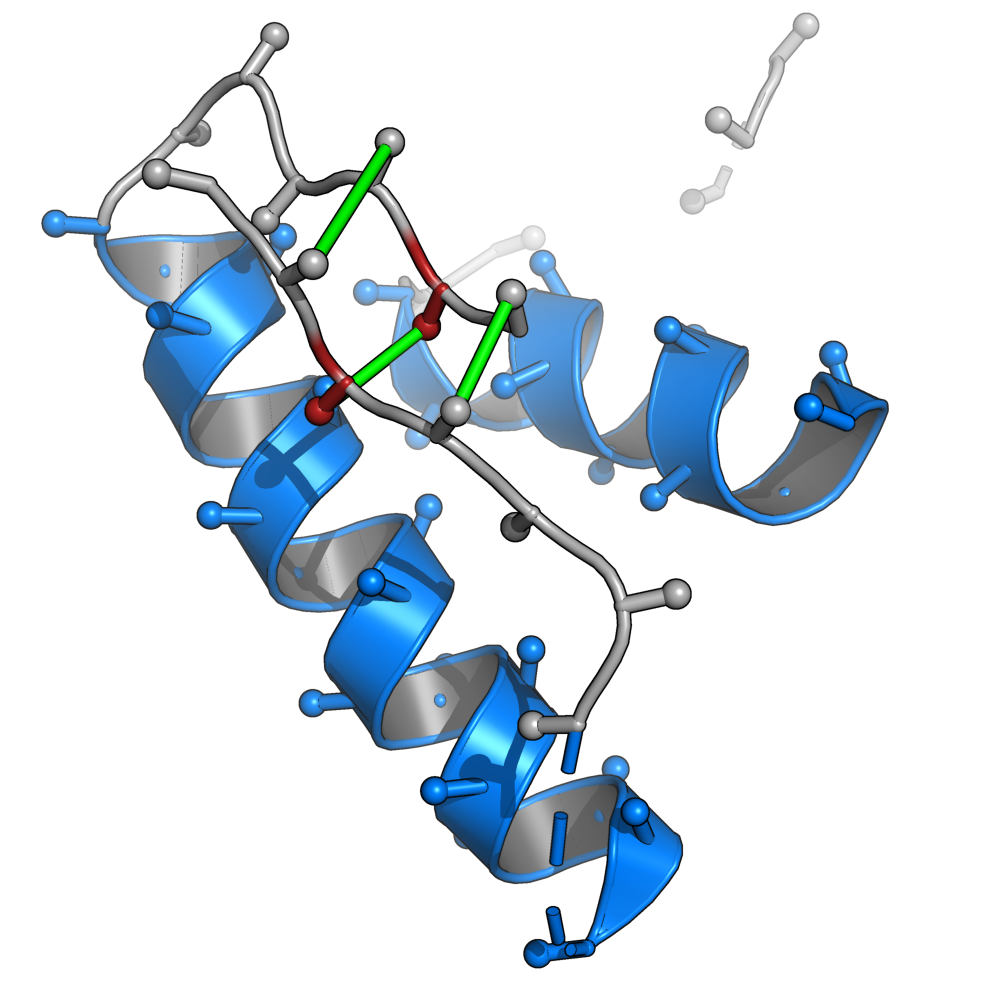
\includegraphics[width=\textwidth]{ample_predictors_1fvg_gbb_phaser_c1_t25_r3_polyAla.png}
    \caption{Successful search model post-PHASER placement for peptide methionine sulfoxide reductase (PDB: 1fvg). BBCONTACTS distance restraints are represented as green lines, \textalpha-helices in blue and \textbeta-strands in red. Secondary structure assignment calculated with STRIDE \cite{Frishman1995-ns}.}
    \label{fig:ample_predictors_1fvg_gbb_phaser_c1_t25_r3_polyAla}
\end{figure}

\section{Discussion}
This study was designed to explore the state-of-the-art metapredictor pipelines for residue-residue contact prediction. The main focus of this work was to distinguish differences in three key parts: raw contact predictions, their use in  ab initio structure prediction and finally the effects on unconventional Molecular Replacement using AMPLE.

Key findings in this study revealed METAPSICOV and PCONSC2 metapredictors to yield the most precise contact predictions regardless of target fold or size. These results are in line with previous findings, which independently confirmed METAPSICOV contact predictions to yield the highest precision across numerous prediction algorithms \cite{Wuyun2016-tx, De_Oliveira2017-yf}. However, work in this study cannot confirm their findings, which demonstrate more precise contact predictions for all-\textbeta\ and mixed \textalpha-\textbeta\ protein targets compared to all-\textalpha\ ones. Several reasons might give insights into this discrepancy: (1) a much smaller sample size was trialled in this study (Wuyun et al.: 680 \cite{Wuyun2016-tx}; de Oliveria et al.: ~3500 \cite{De_Oliveira2017-yf}); (2) the targets were chosen to deliberately sample various alignment depths including relatively low Neff (\textless 200) values; (3) only final contact predictions were analysed as part of this work, thus benefiting from post-prediction consensus finding and contact map processing through unsupervised machine-learning algorithms.

Furthermore, we demonstrated in this study that two similar ROSETTA energy functions yield different structure prediction results. The FADE function on average achieves more accurate structure predictions compared to the SIGMOID one. This result seems surprising at first; however, a closer inspection of each of the energy function parameters gives possible insights into the reasons for the different outcomes. The FADE energy function defines both a maximum and minimum distance. The FADE energy function also does not consider amino acid-specific distances while the SIGMOID function does \cite{Kamisetty2013-bs}. Furthermore, a custom weight factor is added for SIGMOID restraints to balance the restraint term in the overall energy term of each decoy (Sergey Ovchinnikov, personal communication). Thus, small changes in each of those definitions could have significant effects on the final structure prediction. Unfortunately, it is out of the scope of this study to explore all variations, and thus results aid primarily as guide for future work and AMPLE users. This study highlighted again the benefits of adding BBCONTACTS predictions to existing contact maps to further restrain \textbeta-rich regions during structure prediction. This work provides further support to work outlined in Chapter XYZ.

Lastly, part of the comparison carried out in this study was aimed specifically at macromolecular crystallographers and, in particular, AMPLE users. Beyond the proof-of-principle study described in Chapter XYZ, this work further illustrates how important additional restraint information can be to increase the chances of unconventional MR success. However, this work also highlighted limitations in the AMPLE routine whereby decoys that were restrained by residue-residue contacts achieved much higher decoy quality compared to unrestrained ROSETTA decoys, yet solved fewer targets. The idea that restrained decoys might benefit from a different kind of processing was further supported by the most successful decoy sets, which were obtained with GREMLIN contact predictions. Given that GREMLIN and ROSETTA decoys achieved similar decoy qualities for a large set, their structure solutions were identical for all of ROSETTA’s successful solutions. GREMLIN decoys outperformed ROSETTA decoys solely on the basis that it acquired highly accurate decoys for one further target, and thus achieved the most structure solutions in this study. 

Therefore, further work is required to identify the optimal strategy for decoy sets with high structural similarities to the native fold. Such work could focus on the recent idea of selecting decoys based on their long-range contact satisfaction \cite{De_Oliveira2017-yf, Ovchinnikov2017-nd} to specifically eliminate the worst decoys, and thus enhance a more fine-grained clustering approach in SPICKER. Alternatively, truncation could be guided by alternative means, such as the importance of each residue in the predicted contact map. Ultimately, it is key to improve the AMPLE protocol to exploit the much higher decoy quality to enhance the user’s chance of success.


\chapter{Decoy subselection for ...}
% % \section{Introduction}

\section{Methods}

\subsection{Target selection}

The dataset for this experiment was compiled of all modelling runs from all targets used in previous studies. All decoy sets restrained with contact predictions from either CCMPRED \cite{Seemayer2014-ml}, MEMBRAIN \cite{Yang2013-lv}, METAPSICOV \cite{Jones2015-wp} or PCONSC2 \cite{Skwark2014-mu} and the FADE energy function were considered. In total, this gave a set of 56 targets with a maximum of four contact predictions each. However, not all predictors were applicable to all targets, such as the \textalpha-helical transmembrane predictor MEMBRAIN \cite{Yang2013-lv} to globular targets. Thus, a final dataset of 113 decoy sets (1,000 decoys each) was created.

\subsection{Decoy subselection}

The precision score of long-range contact pairs ($\geq24$ residues sequence separation) was calculated for every decoy in every decoy set using ConKit (see Chapter XYZ). Subsequently, decoy sets were reduced for Molecular Replacement trials. Four different algorithms were used: \textit{NONE}, \textit{LINEAR}, \textit{SCALED}, and \textit{CUTOFF}. The \textit{NONE} algorithm accepted all 1,000 decoys and left the original set unchanged, which is identical to the current AMPLE approach. The \textit{LINEAR} algorithm sliced a decoy list removing the 500 decoys satisfying the least number of long-range contacts. For the \textit{SCALED} algorithm, each long-range satisfaction score was divided by the set's average score, and only decoys with scores $\geq0.5$ kept. The \textit{CUTOFF} algorithm excluded all decoys with a long-range satisfaction score of $<0.287$, a hard-coded threshold identified by \cite{De_Oliveira2017-yf} Thus, for every starting decoy set, we obtained four different decoy sets for Molecular Replacement trials using AMPLE.

\subsection{Molecular Replacement}
%
% For the Molecular Replacement trials, a modified version of AMPLE was used. The modified version created ensemble search models for all 10 clusters. Trialling decoys from all 10 clusters was aimed to broaden the search space by including more conformations. Simultaneously, previous results suggested that polyalanine side-chain treatment by itself was nearly as good as all three side-chain treatments. Thus, to reduce the number of ensemble search models to trial, the most-reliable side-chain treatment was excluded. Similarly, the 2\AA subclustering radius appeared to be redundant in almost all cases, and thus this set of ensembles was also removed. Additionally, clustering was performed using a modified version of Spicker, which clusters decoys using TMscore values instead of RMSD values. Although at an increased runtime, this modification has shown to be beneficial to the clustering step (Jens MH Thomas; PhD Thesis). All modifications explained here were made publicly available in AMPLE v1.2.0 and CCP4 v7.0.32.
%
% To trial the different subselection algorithms, we decided to trial one contact prediction decoy set for 21 targets, which created a total of 63 AMPLE runs (three for each set). The target and resulting decoy sets were identical to the one published by @Simkovic2016. Besides the modifications outlined above, AMPLE was run with default settings.
%
\section{Results}

In this experiment, we assessed the value of subselecting sets of 1,000 decoys to AMPLE's cluster-and-truncate approach. Decoys were subselected using one of four algorithms, namely \textit{NONE}, \textit{LINEAR}, \textit{SCALED} or \textit{CUTOFF}. Each algorithm considered the long-range contact satisfaction in a decoy and used it to exclude different numbers from the original set.

\subsection{Long-range contact predictions are indicative of model quality}

\subsection{Different subselection modes yield different final decoy sets}

% \section{Discussion}


\chapter{Alternative \textit{ab initio} structure prediction algorithms for AMPLE}
% \input{chapters/chapter08}

\chapter{Fragments for MR ...}
% % \section{Introduction}
%
% - \texit{Ab initio} structure prediction is a balancing act between time spent to generate decoys and the quality of the final decoy set
% - \texit{Ab initio} structure prediction can only predict accurate structures with a subselection of fragments collective capturing the overall target fold
%
% - AMPLE requires decoys with the overall accurate fold yet enough diversity in the set to truncate to the conserved core
% - AMPLE typically succeeds with small to medium size fragments relative to the target sequence (20-50\%)
%
% This bares the question whether fragments extracted for \textit{ab initio} structure prediction are sufficient as \gls{mr} search models. This stems primarily on the assumption that fragment picking algorithms can identify fragments based on sequence features that are structurally similar to a sequence position in our target.
%
% - Something about the addition of contacts as unique feature for further identifying correct fragments
% - Something about differences to other fragment-\gls{mr} approaches

\section{Methods}
\subsection{Target selection}
Targets were manually chosen using favourable cases for this proof-of-principle study, i.e. resolution was chosen to be ~1.5\AA, target chain lengths were $<150$ residues, and only a single molecule is present in the asymmetric unit (\cref{table:ample_flib_target_properties}).

\begin{table}[H]
  \centering
  \caption{Overview of Flib target properties.}
  \label{table:ample_flib_target_properties}
  \begin{tabularx}{\textwidth}{X X X X X X}
      \hline
      \textbf{Target} & \textbf{Fold} & \textbf{Chain Length} & \textbf{Resolution (\AA)} & \textbf{Nmol/ASU} &
\textbf{Space Group} \\ 
      \hline
      1aba & mixed \textalpha-\textbeta & 87    & 1.45 & 1      & P $2_1$ $2_1$ $2_1$   \\
      1lo7 & mixed \textalpha-\textbeta & 141   & 1.50 & 1      & I $2$ $2$ $2$         \\
      1u06 & all-\textbeta              & 62    & 1.49 & 1      & P $2_1$ $2_1$ $2_1$   \\
      5nfc & all-\textbeta              & 147   & 1.59 & 1      & P $2_1$ $2_1$ $2_1$   \\
      \hline
  \end{tabularx}
\end{table}

\subsection{Fragment picking using Flib}
Fragments for this study were picked using the Flib algorithm \cite{De_Oliveira2015-ba}. 

Flib requires four inputs: the predicted secondary structure, predicted torsion angles, predicted residue-residue contact prediction and a copy of the \gls{pdb}. The secondary structure for each target was predicted using PSIPRED v4.0 \cite{Jones1999-fi} with default parameters. The torsion angles were predicted using SPIDER2 \cite{Heffernan2015-wp} with default parameters, and residue-residue contact pairs using METAPSICOV v1.04 \cite{Jones2015-wp} with default parameters. HHBLITS v2.0.16 \cite{Remmert2011-ze} with database version \texttt{uniprot20\_2016\_02} was used by METAPSICOV to generate the \gls{msa} for contact prediction of each target sequence. BLASTp v2.2.31+ \cite{Altschul1990-nc,Camacho2009-ue} was used by PSIPRED with the UNIPROT database version \texttt{uniref90-2016\_06}. The local copy of the \gls{pdb} for fragment picking was downloaded on August 11, 2016.

Two modifications were made to the default Flib v1.01 (\url{https://github.com/sauloho/Flib-Coevo}) protocol. The first focuses on exclusion of fragments with $>90$\% helical content (assigned by DSSP \cite{Frishman1995-ns}). The second modification was to allow fragments with \gls{rmsd} $>10.0$\AA\ to be considered.

Two-hundred fragments were picked per target sequence position. Top-$L$ or $L/2$ contact pairs were considered from both METAPSICOV STAGE 1 and STAGE 2 predictions with a minimum sequence separation of either 6 or 12 residues. Helical fragments were either in- or excluded and only fragments with length between 6 or 12 residues up-to 63 residues considered. Overall, this generated 16 fragment libraries per target.

Each fragment library was then filtered to remove homologs. Hereby, BLASTp and HHpred \cite{Soding2005-sx} searches were conducted to identify homologous PDB entries. The BLASTp search was performed identically to \cite{De_Oliveira2015-ba}. The HHpred search parameters were identical to the MPI-Toolkit \cite{Biegert2006-ny} webserver version (\url{https://toolkit.tuebingen.mpg.de/}). Fragments derived from PDB entries identified by BLASTp and HHpred (probability score of $\geq20.0$) were excluded from the fragment libraries.

All fragments per target were then grouped by their length. Subsequently, they were ranked twice by Flib scores and \gls{rmsd} values, and the best fragment selected. Fragments of the same template structure consisting of the same region with varying flanking residues were kept, if they were ranked top for each fragment length group. Finally, the coordinates for the selected fragments were extracted and two files created for each, one containing the backbone atoms and the other containing all atoms.

\subsection{\acrlong{mr} in MrBUMP}
The previously extracted fragments were subjected to the \gls{mr} pipeline MrBUMP \cite{Keegan2008-hk}. The latter uses PHASER \cite{McCoy2007-bf} for \gls{mr}, REFMAC5 \cite{Murshudov2011-we} for refinement and SHELXE \cite{Thorn2013-ir} for density modification and main-chain tracing. MrBUMP default parameters were used with exception of the PHASER RMS estimate. \gls{mr} was attempted for each coordinate file with a PHASER RMS value of 0.1, 0.6, and 1.0.

The \gls{mr} success for each search model was assessed by SHELXE scores only, whereby a \gls{cc} score of $\geq25.0$ combined with an \gls{acl} score of $\geq10.0$ is required.


\section{Results}
\subsection{Precision of Flib dependency data}
The first part of this study is to analyse the data dependencies required by the Flib fragment picking algorithm. This analysis is important given that the Flib fragment picking heavily relies on the individual features in the selection and scoring of each individual fragment \cite{De_Oliveira2015-ba}. Poor data at this stage could lead to poor fragments unsuitable for \gls{mr} trials given that high accuracy, i.e. an low \gls{rmsd} value between the search model and target, is required.

The secondary structure prediction highlighted high precision between each target's prediction and the DSSP-assigned \cite{Frishman1995-ns} secondary structure of the target reference structure (\cref{fig:ample_flib_psipred}). The three targets with \gls{pdb} identifiers 1aba, 1lo7 and 1u06 have secondary structure predictions with a precision of $>72$\%. The fourth target, 5nfc, shows comparatively poor precision of 52.4\%. However, almost all secondary structure features are correctly identified.

\begin{figure}[H]
	\centering
	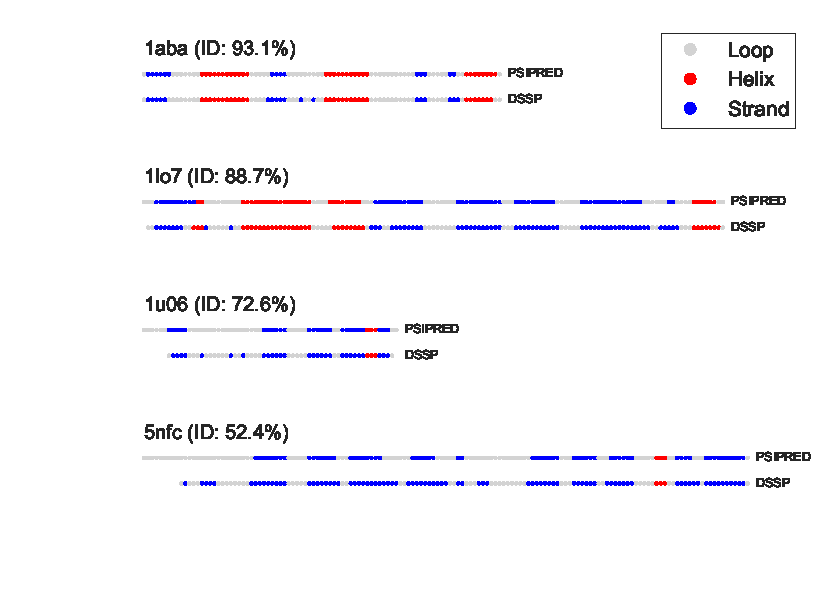
\includegraphics[width=\textwidth]{ample_flib_psipred.pdf}
	\caption[PSIPRED schema for Flib targets]{Schematic comparison of PSIPRED \cite{Jones1999-fi} secondary structure prediction and DSSP \cite{Frishman1995-ns} assignment. Percentage identity is provided next to each identifier.}
	\label{fig:ample_flib_psipred}
\end{figure}

The contact prediction data for METAPSICOV STAGE 1 and STAGE 2 predictions demonstrate the high precision scores achievable by this algorithm (\cref{table:ample_flib_contact_precision}). In this study, the top contact pairs at cutoffs \textit{L} and \textit{L/2} were provided to the Flib algorithm. All targets have precision scores for both sets of predictions at both cutoff levels of $>0.6$ (\cref{table:ample_flib_contact_precision}).

\begin{table}[H]
  \centering
  \caption[Contact prediction summary for Flib targets]{Precision scores for METAPSICOV \cite{Jones2015-wp} STAGE 1 and STAGE 2 contact predictions. Jaccard index calculated for the same contact pairs between METAPSICOV STAGE 1 and STAGE 2 predictions.}
  \label{table:ample_flib_contact_precision}
  \begin{tabularx}{\textwidth}{X X X X X X X}
      \hline
	  \multirow{2}{*}{\textbf{Target}} & \multicolumn{3}{c}{\textbf{\textit{L/2} contact pairs}} & \multicolumn{3}{c}{\textbf{\textit{L} contact pairs}} 	\\ \cline{2-7}
	  							&  	STAGE 1	& 	STAGE 2	& 	Jaccard 	& 	STAGE 1 	& 	STAGE 2 	& 	Jaccard	 	\\
	  \hline
	  1aba						&	0.884	&	0.884	&	0.303	&	0.713	&	0.759	&	0.513		\\
	  1lo7						&	0.857	&	0.957	&	0.308	&	0.738	&	0.837	&	0.446		\\
	  1u06						&	0.839	&	0.806	&	0.378	&	0.710	&	0.787	&	0.459		\\
	  5nfc						&	0.822	&	0.836	&	0.327	&	0.619	&	0.762	&	0.434		\\ 
	  \hline
  \end{tabularx}
\end{table}

Given the two prediction files, both show localised clusters of contact pairs suggesting
 secondary structure features found in the native protein structures (\cref{fig:ample_flib_cmaps}). However, METAPSICOV STAGE 1 predictions show a much higher frequency of singleton contact pairs, i.e. ones without a neighbouring contact pair.

\begin{figure}[H]
	\centering
	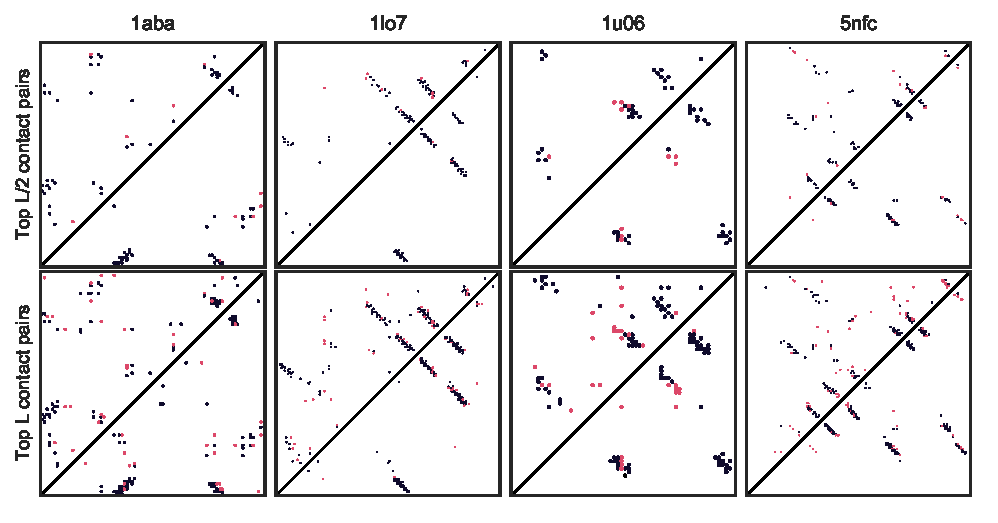
\includegraphics[width=\textwidth]{ample_flib_cmaps.pdf}
	\caption[Contact map comparison for Flib targets]{Comparison of $L/2$ and $L$ correctly (gray) and incorrectly (pink) predicted contact pairs for four Flib targets. Contacts were predicted using METAPSICOV STAGE 1 (top left) and STAGE 2 (bottom right) \cite{Jones2015-wp}. True and false positive contact pairs were identified using a 8\AA cutoff between C\textalpha\ (C\textbeta\ in case of GLY) atoms of a reference crystal structure.}
	\label{fig:ample_flib_cmaps}
\end{figure}

An analysis of the absolute difference of torsion angles between the SPIDER2 \cite{Heffernan2015-wp} prediction and a corresponding reference crystal structure highlight accurate predictions for three of four targets (\cref{fig:ample_flib_spider2}). The largest \gls{mae} of \textphi-angles across the four target sequences is $24.347^{\circ}$, and the largest \gls{mae} of \textpsi-angles is $45.459^{\circ}$ (\gls{mae} values for \gls{pdb} entry 1u06). The smallest \textphi-\gls{mae} is $13.822^{\circ}$ (\gls{pdb}: 1aba) and smallest \textpsi-\gls{mae} is $17.273^{\circ}$ (\gls{pdb}: 1lo7). Segments in sequence space with regular secondary structure, as predicted by PSIPRED \cite{Jones1999-fi}, result primarily in low \gls{mae} of torsion angles. In contrast, unstructured regions highlight much larger \gls{mae} values indicating the difficulty of predicted these regions. Noticeably, the \textpsi-\gls{mae} appears to be much larger in those regions than the \textphi-\gls{mae} for the same residue.

\begin{figure}[H]
	\centering
	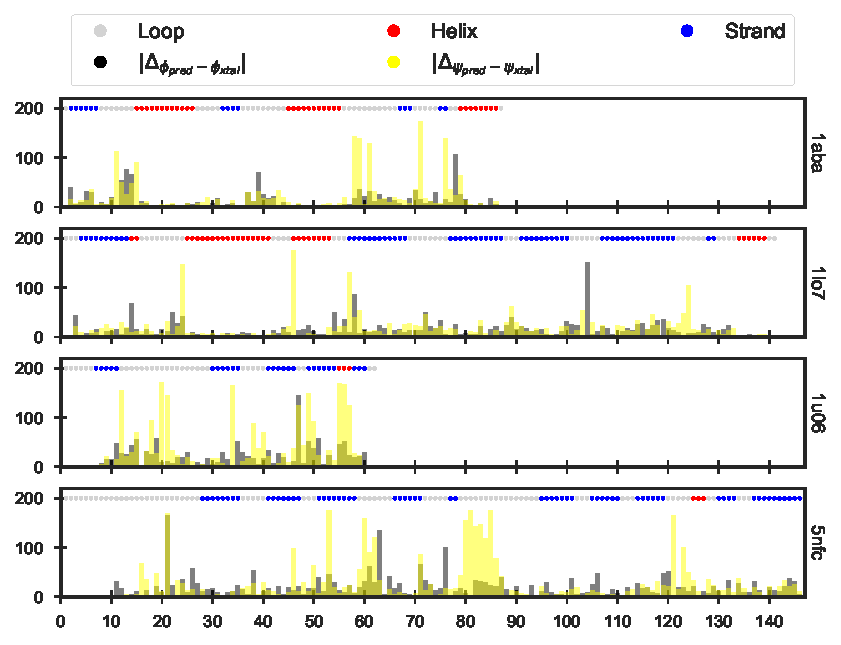
\includegraphics[width=\textwidth]{ample_flib_spider2.pdf}
	\caption[SPIDER2 torsion angle prediction analysis of Flib targets]{Comparison of \gls{mae} of torsion angles predicted by SPIDER2 and extracted from a corresponding \gls{pdb} structure. PSIPRED \cite{Jones1999-fi} secondary structure prediction provided alongside the \gls{mae} values.}
	\label{fig:ample_flib_spider2}
\end{figure}

\subsection{Flib fragment picking}

Sixteen Flib fragment libraries were picked for each protein target in this study. Each fragment library consisted of one permutation given altering input paramaters and contact prediction files.

Across all four targets, the Flib algorithm selected a total of 8,548,775 fragments (\cref{table:ample_flib_frag_summary}). The fragment libraries show similar statistics across the four protein targets despite the diversity in fold and chain lengths. The Flib score average falls at ~3,200 Flib score units with an average 9.0\AA\ \gls{rmsd}. Fragments for the alpha-spectrin SH3 domain (\gls{pdb} ID: 1u06) scored the lowest mean Flib score with 3035.50 units; however, the same target scored the worst by mean \gls{rmsd} with an average of 9.48\AA. In contrast, fragments picked for the sequence of the bacteriophage T4 glutaredoxin (\gls{pdb} ID: 1aba) achieved the best mean \gls{rmsd} of 7.85\AA\ given the second highest mean Flib score of 3217.49 units (\cref{table:ample_flib_frag_summary}).

\begin{table}[H]
  \centering
  \scriptsize
  \caption[Flib fragment characterics across four protein targets]{Summary of fragment statistics for Flib libraries selected for four protein targets. Count\textsubscript{H} corresponds to the count of fragments extracted from homologs.}
  \label{table:ample_flib_frag_summary}
  \begin{tabularx}{\textwidth}{X X X X X X X X X}
      \hline
      \multirow{2}{*}{\textbf{Target}} & \multirow{2}{*}{\textbf{Count}} & \multirow{2}{*}{\textbf{Count\textsubscript{H}}} & \multicolumn{3}{c}{\textbf{Flib score}} & \multicolumn{3}{c}{\textbf{\gls{rmsd}}} \\ \cline{4-9}
      		&			&			& Median 	& Mean 		& Sigma 	& Median 	& Mean 	& Sigma \\
      
      \hline
	  1aba	& 2,094,332	& 45,193	& 3061.05	& 3217.49	& 1405.71	& 7.70		& 7.85	& 3.81	\\
  	  1lo7  & 2,501,675	& 23,416	& 3187.44	& 3372.06	& 1497.49	& 9.00		& 9.43	& 4.61  \\
      1u06  & 1,136,435	& 60,456	& 2902.68	& 3035.50	& 1306.17	& 9.51		& 9.48	& 3.94	\\
      5nfc  & 2,816,333	& 48,839	& 2982.69	& 3127.00	& 1316.56	& 8.89		& 9.16	& 4.18	\\ 
      \hline
      Total	& 8,548,775	& 177,904	& 3049.31	& 3208.72	& 1397.20	& 8.68		& 8.96	& 4.25	\\ 
      \hline
  \end{tabularx}
\end{table}

A split of the per-target fragment libraries into their distinct conditions highlights the improved library quality of certain conditions with regards to the mean Flib score and \gls{rmsd} (\cref{fig:ample_flib_flibcond}). In particular, top-$L$ (6 residues sequence separation) METAPSICOV STAGE 1 contact predictions yielded the lowest for both metrics across all targets, which suggests this condition to be the most favourable for picking fragments. A comparison of the sequence separation, i.e. using all contact pairs or medium- and long-range ones only, strongly suggests much lower and thus more favourable scores for using all contact pairs. A very similar difference is noticeable for METAPSICOV STAGE 2 contact predictions (\cref{fig:ample_flib_flibcond}). Independent of the starting contact prediction, the most favourable condition for selecting fragments using Flib uses top-$L$ contact pairs with 6 residues sequence separation. The exclusion of idealised \textalpha-helical fragments did not affect the overall Flib score and \gls{rmsd} greatly ($max \Delta_{Flib}=25.87; max \Delta_{RMSD}=0.06$).

\begin{figure}[H]
	\centering
	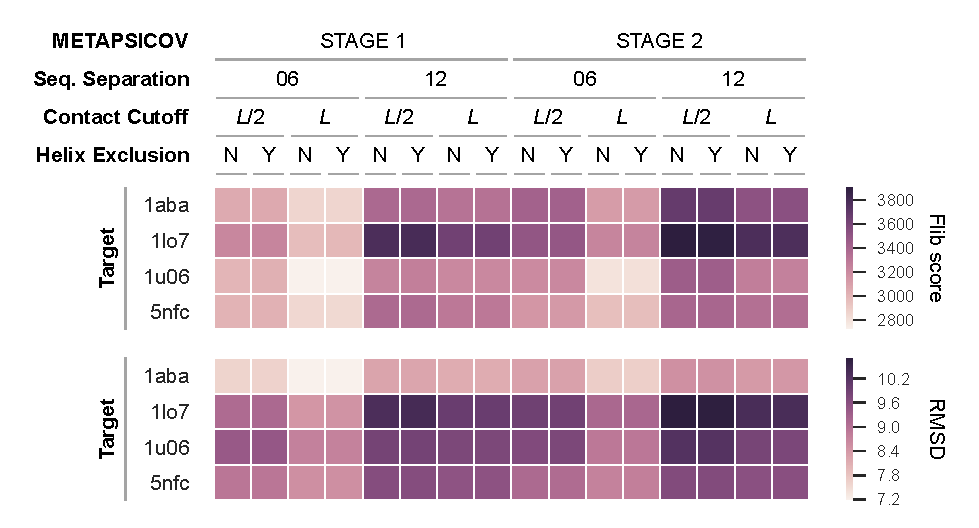
\includegraphics[width=\textwidth]{ample_flib_flibcond.pdf}
	\caption[Flib fragment library comparison]{Flib fragment library comparison for four targets highlighting the differences in mean Flib score and \gls{rmsd} by starting with different subsets of contact predictions. $L$ refers to the number of residues per target sequence. $Y$ refers to idealised \textalpha-helical fragment exclusion during fragment picking; $N$ refers to treating those fragments like all others.}
	\label{fig:ample_flib_flibcond}
\end{figure}

\subsection{Flib fragment selection for \acrlong{mr}}

One of the most important aspects of bypassing \textit{ab initio} structure prediction and using the relevant fragments directly as \gls{mr} search models is the selection of the fragments with the highest similarity between fragment and target structure. The Flib score - a cumulative metric judging the quality of a fragment - is the most obvious feature; however, it is unknown to-date whether a correlation between the Flib score and the fragment \gls{rmsd} exists. Taking all non-homologous fragments in this study, a first attempt was made to identify a correlation between a fragment's Flib score and \gls{rmsd}. The results presented here indicate towards a positive correlation between the Flib score and the corresponding fragment \gls{rmsd} for almost all fragments across the different target fragment libraries (\cref{fig:ample_flib_flibrelat}). However, a small fraction of fragments appear as outliers, not fitting the correlation of lower Flib scores corresponding to lower \gls{rmsd} values. On average, 0.2\% of fragments per library are contained in this outlier set.

\begin{figure}[H]
	\centering
	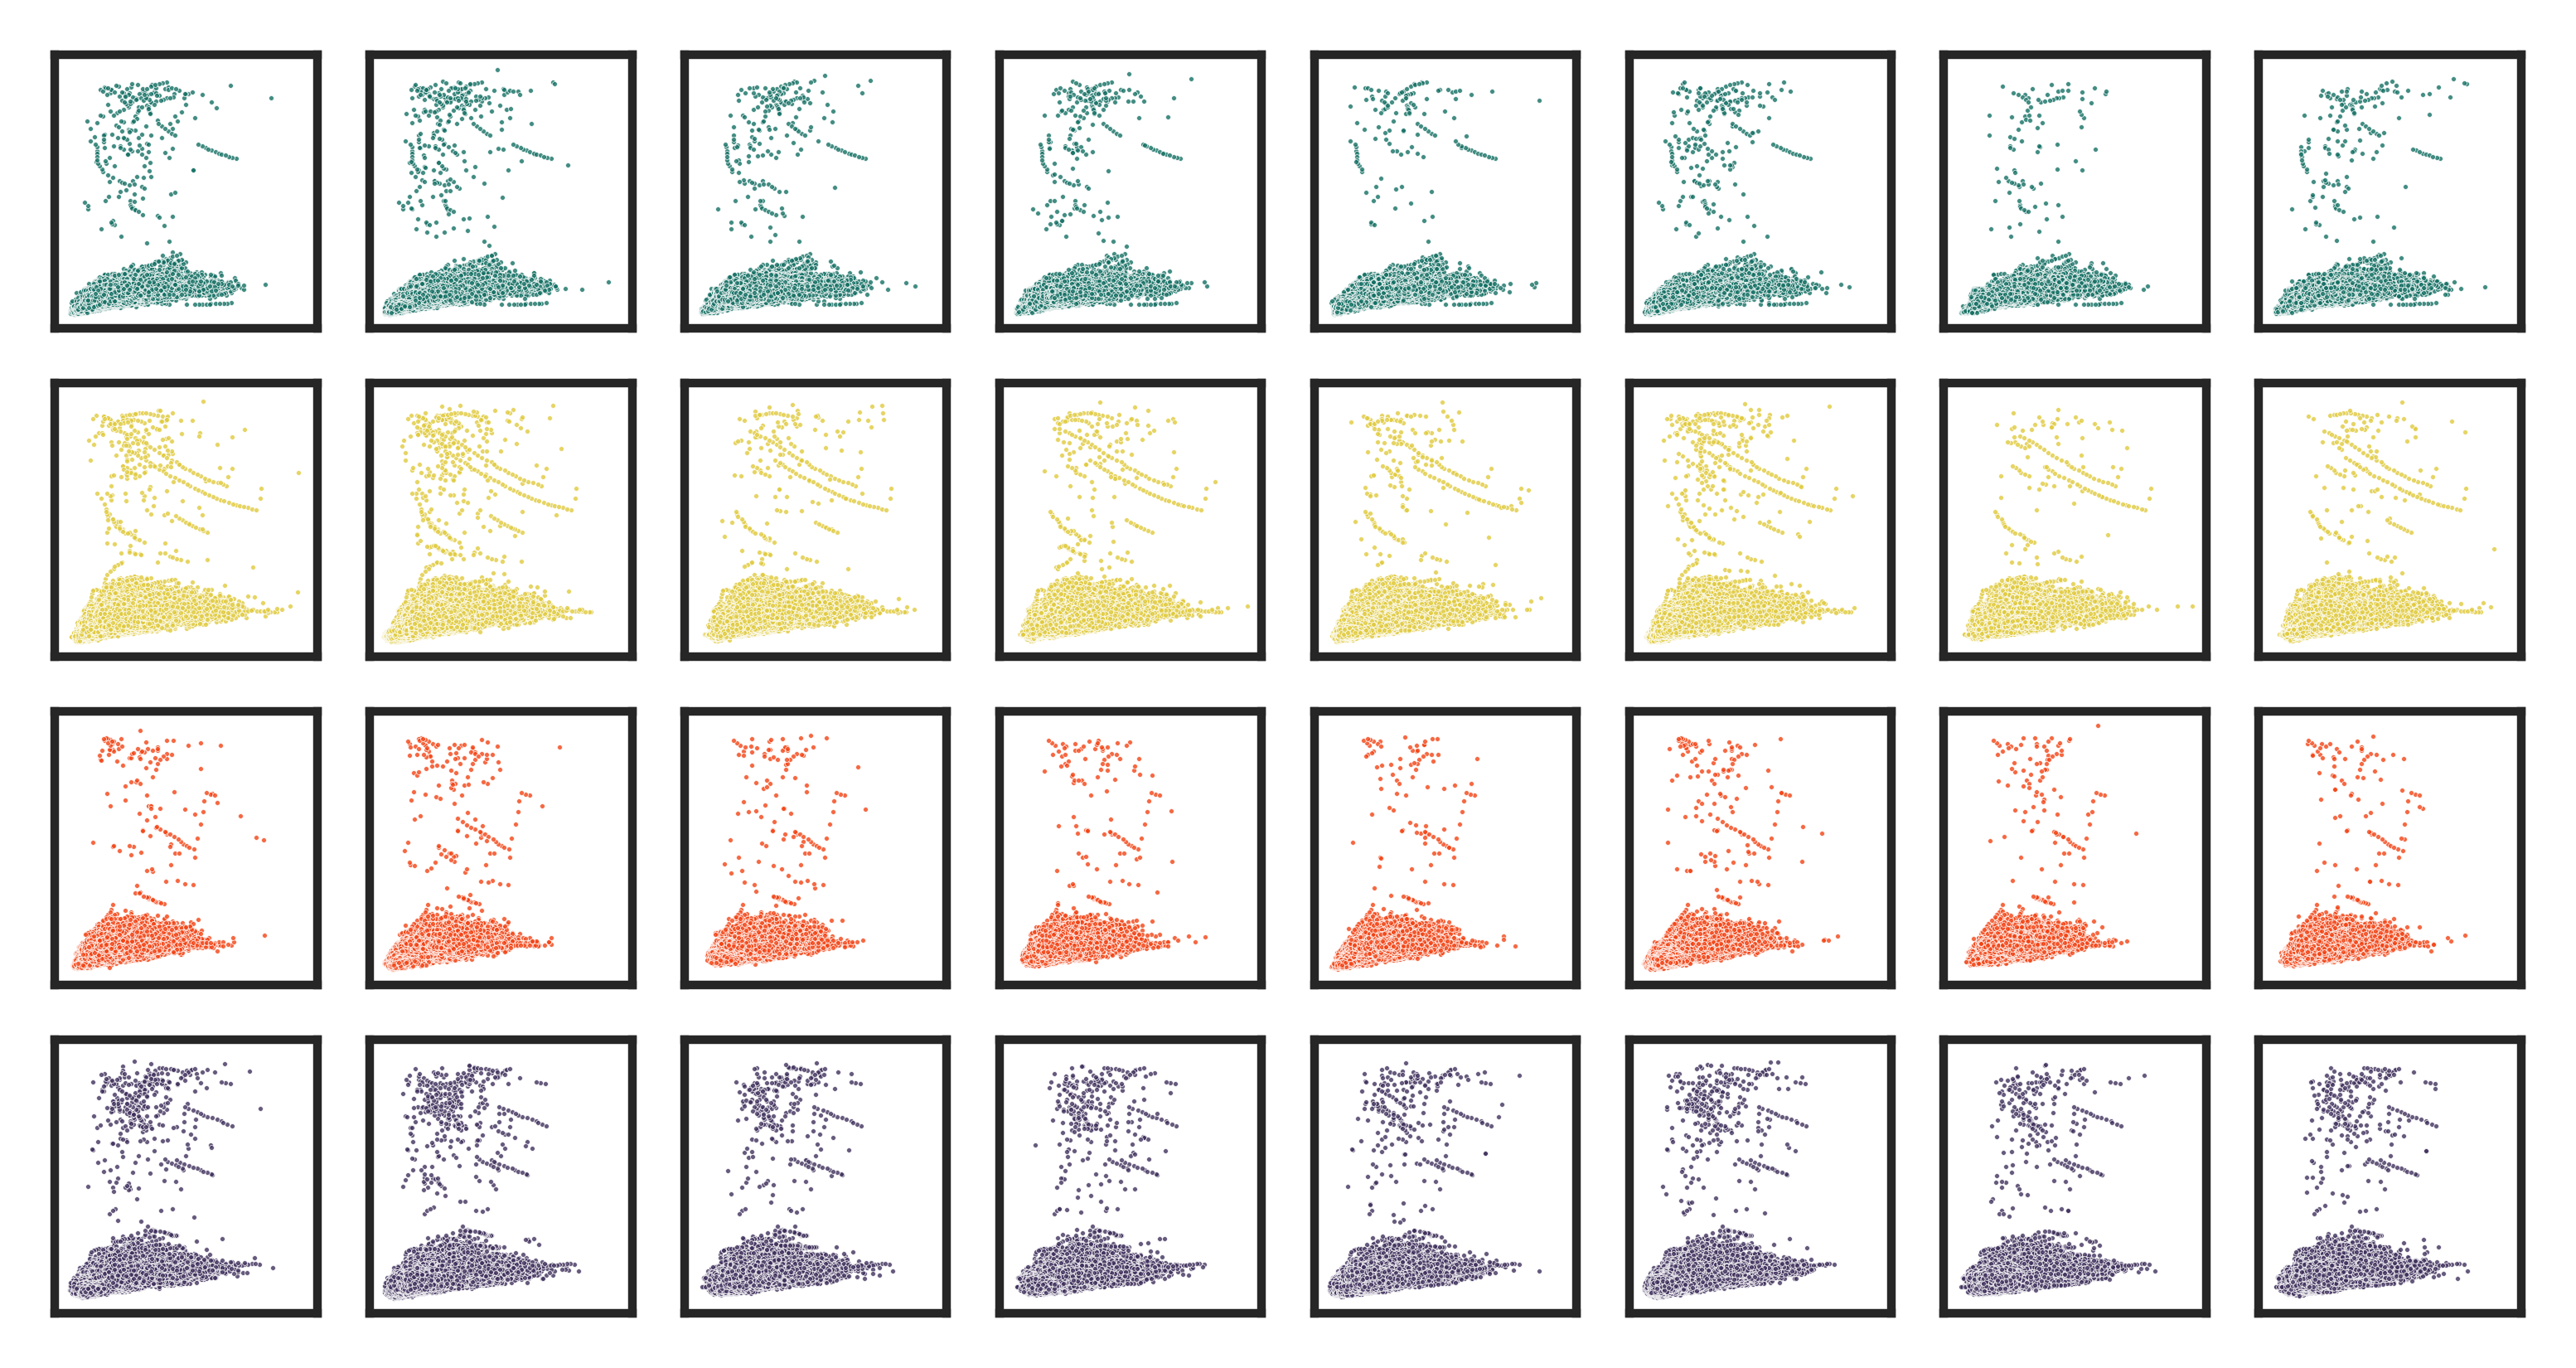
\includegraphics[width=\textwidth]{ample_flib_flibrelat.png}
	\caption[Correlation analysis for Flib score and \gls{rmsd}]{Scatterplot highlighting the positive correlation between fragment Flib scores (x-axes) and \gls{rmsd} values (y-axes). Four targets are illustrated: 1aba (green), 1lo7 (yellow), 1u06 (orange), and 5nfc (purple). Each column represents a different fragment picking strategy, and no fragment illustrated correpsonds to an idealised \textalpha-helix.}
	\label{fig:ample_flib_flibrelat}
\end{figure}

An analysis of the outliers for characteristics that would allow for their exclusion showed the randomness of their occurrence. These fragments contain all secondary structure types, span the entire target sequence and consist of a great range of peptide lengths. Furthermore, they occur in all fragment libraries, irrelevant of their original picking strategy. The only characteristic, which would be impossible to use \textit{a priori} is the fragments' \gls{rmsd} values, which are $>30$\AA. However, it is worth noting that the minimum Flib score in the outlier fragment set and the remaining fragment sets are distinctly different. The outliers' minimum extracted from all fragment sets is 795.62 Flib score units. In comparison, fragments with \gls{rmsd} $\leq30$\AA\ have a minimum \gls{rmsd} of 72.16, which suggests that the outlier fragments might not make it in the final selection.

% - no outliers made it to the final set
% - larger fragments have inherently lower Flib scores but also lower RMSD
% - three large fragments have high Flib but low-ish RMSD

\chapter{Single model approach using AMPLE's cluster-and-truncate approach}
% \input{chapters/chapter10}

\chapter{Software developments}
% \input{chapters/chapter11}

\chapter{Conclusion}
% \section{Conclusion}
The successful disentanglement of direct and indirect residue contacts in contact prediction revolutionised many aspects of Structural Bioinformatics research \cite{Simkovic2017-xs}. Successful applications of contact information range from accurately defining domain boundaries \cite{Sadowski2013-zu} to identifying druggable protein-protein interfaces \cite{Bai2016-sw}. Although many such applications have been highlighted over the last few years \cite{Simkovic2017-xs}, few concerned the topic of \gls{mr} in X-ray crystallography. In this thesis, work was presented that made first attempts to apply contact information to explore some of its application spectrum in \gls{mr}.

The use of contact information in \textit{ab initio} protein structure prediction allowed researchers to predict the structure of many previously unknown protein folds based on their sequence alone \cite[e.g.,][]{Marks2011-os,Michel2014-eg,Kosciolek2014-bt,Ovchinnikov2015-tn,Ovchinnikov2016-jj,Michel2017-xh,De_Oliveira2017-sg,Ovchinnikov2017-nd,Wang2017-rx}. The major benefit of adding such information was to reduce the conformational search space, which allowed more challenging folds to be sampled correctly. Work presented in \cref{chap:proof_of_principle,chap:rosetta_energy_functions,chap:alternate_abinitio_protocols} further confirm such findings. More importantly, the presented results highlight that the modelling algorithm ROSETTA is very sensitive to the way contact information is introduced into the ROSETTA folding protocol. Two important examples include the up-weighting of \textbeta-strand contacts and the choice of energy function used to ``reward'' satisfied contacts. Furthermore, work in \cref{chap:alternate_abinitio_protocols} highlights that fragment-based structure prediction algorithms may no longer be essential for accurate structure prediction. CONFOLD2, a fragment-independent algorithm, predicts the protein structure using secondary structure and contact information alone, which provided models of comparable accuracy to the state-of-the-art ROSETTA.

Beyond the prediction of protein structures, a major focus of the presented research centred on the benefit of such improved structure predictions in unconventional \gls{mr}. In-line with prior expectations, better structure predictions yield more \gls{mr} structure solutions. In particular, previous weakpoints of the AMPLE routine --- the target chain length and fold --- can successfully be addressed with contact-guided structure predictions. Some examples for which structure solutions were obtained exceed 200 residues in chain length, whilst many others contain large proportions of \textbeta-structure. Nevertheless, simply adding contact information to \textit{ab initio} protein structure prediction is not sufficient to solve all trialled targets. Thus, further research, outlined in \cref{chap:ample_decoys}, explored one way of incorporating contact information in the AMPLE processing pipeline. Contact information was used to estimate the similarity of a predicted decoy to its native structure, by means of scoring its long-range contact satisfaction. Exclusion of the worst decoys by this metric prior to clustering allowed more fine-grain sampling in AMPLE, which turned unsuccessful decoy sets into ones from which the native structure can be eludicated.

A further topic of research concerned the use of supersecondary structure elements or subfolds as \gls{mr} search models. The default mode in AMPLE currently relies on computationally expensive \textit{ab initio} structure predictions. Since contact predictions have reached sufficient quality for protein families with many known sequences, such information could be used to identify matching subfolds in other, unrelated protein structures. In \cref{chap:ample_flib}, a new hybrid approach demonstrated the successful implementation of such an idea. Although imperfect at this stage, several examples highlighted the successful identification of such subfolds and subsequently successful \gls{mr} structure solution.

\section{Outlook}
In this thesis first applications of predicted contact information in \gls{mr} were presented. Despite the already promising results, this area of research is still in its infancy and a great number of potentially promising routes remain unexplored. Earlier studies by \textcite{Rigden2002-mf} and \textcite{Sadowski2013-zu} demonstrated the successful application of residue contacts to identify domain boundaries. Although unexplored to-date, precise domain boundary predictions could be applied for better domain boundary definitions in \textit{ab initio} structure prediction to avoid sampling of terminal loops and linkers, and thus improve protein structure prediction quality. Furthermore, contact information was used to improve the AMPLE pipeline with respect to excluding poorly predicted decoys. However, the AMPLE ensemble generation pipeline might additionally benefit from contact information to aid the driving of the truncation procedure. For example, contact data could be used to rank individual residues by their contribution to a contact network, similar to \cite{Parente2015-mv}, and truncation driven by the rank order. Additionally, contact prediction might be used in the context of identifying alternative conformational states \cite{Hopf2012-zl,Jana2014-rw,Sfriso2016-ml,Morcos2013-ks, Sutto2015-ck}, which AMPLE could exploit to identify conserved residues between both states and truncate to this conserved core, or attempt remodelling after successful disentanglement of state-dependent contact pairs and try both conformations separately as ensemble search models. Besides the application of contact data in protein structure prediction, other alternatives need to be considered too. Recently, first tools were developed to match predicted contact maps to ones extracted from protein structures \cite{Buchan2017-ox,Ovchinnikov2017-nd}. It might be of interest to investigate how search models, such as distant homologs, could be identified by sequence searches aided with contact map matching. 

%
% \appendix
% \chapter{Appendix Title}
% 
\begin{sidewaystable}
    \footnotesize
    \centering
    \caption{Summary of the ORIGINAL dataset.}
    \label{table:appendix_dataset_original}
    \begin{tabularx}{\textheight}{ t b t t t t t t t s t }
        \hline
        \textbf{\gls{pdb} ID} & \textbf{Molecule}	& \textbf{Resolution (\AA)}	& \textbf{Space Group}	& \textbf{Chain ID}	& \textbf{Chain Length}	& \textbf{Molecules per ASU}	& \textbf{Matthew's Coefficient}	& \textbf{Solvent Content (\%)}	& \textbf{Fold}	& \textbf{Citation}	\\
        \hline
        1a6m		&	Oxy-myoglobin											&	1.00		&	P$2_1$			& A	&	151	&	1	&	1.90		&	36.00	&	all-\textalpha				& \cite{Vojtechovsky1999-nn}	\\
        1aba		&	T4 glutaredoxin											&	1.45		&	P$2_1 2_1 2_1$	& A	&	87	&	1	&	2.22		&	44.62	&	mixed \textalpha/\textbeta	& \cite{Eklund1992-gz}			\\
        1bdo		&	Biotinyl domain of acetyl-coenzyme A carboxylase		&	1.80		&	P$2_1 2_1 2$	& A	&	80	&	1	&	2.48		&	49.00	&	all-\textbeta				& \cite{Athappilly1995-yu}		\\
        1bkr		&	Calponin Homology (CH) domain from \textbeta-spectrin	&	1.10		&	P$2_1$			& A	&	109	&	1	&	2.04		&	39.80	&	all-\textalpha				& \cite{Banuelos1998-jk}		\\
        1chd		&	CheB methylesterase domain								&	1.75		&	P$3_2 2 1$		& A	&	203	&	1	&	2.35		&	47.65	&	mixed \textalpha/\textbeta	& \cite{West1995-dp}			\\
        1e0s		&	G-protein Arf6-GDP										&	2.28		&	P$6_1 2 2$		& A	&	174	&	1	&	2.18		&	37.00	&	mixed \textalpha/\textbeta	& \cite{Menetrey2000-nw}		\\
        1eaz		&	Phosphoinositol (3,4)-bisphosphate PH domain			&	1.40		&	C$2 2 2_1$		& A	&	125	&	1	&	2.48		&	48.00	&	mixed \textalpha+\textbeta	& \cite{Thomas2001-uf}			\\
        1hh8		&	N-terminal region of P67Phox							&	1.80		&	P$3_1$			& A	&	213	&	1	&	2.71		&	45.00	&	all-\textalpha				& \cite{Grizot2001-ju}			\\
        1kjl		&	Galectin-3 domain										&	1.40		&	P$2_1 2_1 2_1$	& A	&	146	&	1	&	2.15		&	42.68	&	all-\textbeta				& \cite{Sorme2005-ln}			\\
        1kw4		&	Polyhomeotic SAM domain									&	1.75		&	P$6_5$			& A	&	89	&	1	&	2.25		&	45.27	&	all-\textalpha				& \cite{Kim2002-vg}				\\
        1lo7		&	4-hydroxybenzoyl CoA thioesterase						&	1.50		&	I$2 2 2$		& A	&	141	&	1	&	2.06		&	40.22	&	mixed \textalpha+\textbeta	& \cite{Thoden2002-id}			\\
        1npu		&	Extracellular domain of murine PD-1						&	2.00		&	P$2_1 2_1 2_1$	& A	&	117	&	1	&	1.67		&	25.80	&	all-\textbeta			& \cite{Zhang2004-zt}			\\
        1pnc		&	Poplar plastocyanin										&	1.60		&	P$2_1 2_1 2_1$	& A	&	99	&	1	&	1.82		&	32.48	&	all-\textbeta				& \cite{Fields1994-zx}			\\
        1tjx		&	Synaptotagmin I C2B domain								&	1.04		&	P$3_2 2 1$		& A	&	159	&	1	&	2.40		&	48.00	&	mixed \textalpha+\textbeta	& \cite{Cheng2004-es}			\\
        1tlv		&	LicT PRD												&	1.95		&	P$3_2 2 1$		& A	&	221	&	1	&	2.80		&	50.00	&	all-\textalpha				& \cite{Graille2005-at}			\\
        2nuz		&	\textalpha-spectrin SH3 domain							&	1.85		&	P$2_1 2_1 2_1$	& A	&	62	&	1	&	2.57		&	52.16	&	all-\textbeta				&								\\
        2qyj		&	Ankyrin													&	2.05		&	P$6_1$			& A	&	166	&	1	&	2.28		&	45.99	&	all-\textalpha				& \cite{Merz2008-aa}			\\
        3w56		&	C2 domain					 							&	1.60		&	I$2$			& A	&	131	&	1	&	2.05		&	40.10	&	all-\textbeta				& \cite{Traore2013-ul}			\\
        4cl9		&	N-terminal bromodomain of Brd4							&	1.40		&	P$2_1 2_1 2_1$	& A	&	127	&	1	&	2.21		&	44.37	&	all-\textalpha				& \cite{Atkinson2014-he}		\\
        4u3h		&	FN3con													&	1.98		&	P$4_1 3 2$		& A	&	100	&	1	&	2.47		&	50.27	&	all-\textbeta				& \cite{Porebski2015-jl}		\\
        4w97		&	KstR2 													&	1.60		&	C$2$			& A	&	200	&	1	&	2.75		&	55.25	&	all-\textalpha				& \cite{Crowe2015-wt}			\\
        \hline
    \end{tabularx}
\end{sidewaystable}

\begin{sidewaystable}
    \footnotesize
    \centering
    \caption{Summary of the PREDICTORS dataset.}
    \label{table:appendix_dataset_predictors}
    \begin{tabularx}{\textheight}{ t b t t t t t t t s t }
        \hline
        \textbf{\gls{pdb} ID} & \textbf{Molecule}	& \textbf{Resolution (\AA)}	& \textbf{Space Group}	& \textbf{Chain ID}	& \textbf{Chain Length}	& \textbf{Molecules per ASU}	& \textbf{Matthew's Coefficient}	& \textbf{Solvent Content (\%)}	& \textbf{Fold}	& \textbf{Citation}	\\
        \hline
        1fcy		& Retinoic acid nuclear receptor HRAR						& 1.30	& P$4_1 2_1 2$		& A	& 236	& 1	& 2.25	& 45.50	&	all-\textalpha				& \cite{Klaholz2000-ux}		\\
        1fvg		& Peptide methionine sulfoxide reductase					& 1.60	& C$1 2 1$			& A	& 199	& 1	& 2.10	& 41.55	&	mixed \textalpha+\textbeta	& \cite{Lowther2000-pp}		\\	
        1gm4		& Cytochrome C3												& 2.05	& P$6_1 2 2$		& A	& 107	& 1	& 2.48	& 50.43	&	all-\textalpha				& \cite{Louro2001-pm}		\\
        1gv8		& N-II domain of ovotransferrin								& 1.95	& P$3_1$			& A	& 159	& 1	& 2.24	& 45.00	&	mixed \textalpha/\textbeta	& \cite{Kuser2002-gh}		\\
        1k40		& FAT domain of focal adhesion kinase						& 2.25	& C$1 2 1$			& A	& 126	& 1	& 2.21	& 44.40	&	all-\textalpha				& \cite{Hayashi2002-gj}		\\
        1oee		& Hypothetical protein YodA 								& 2.10	& C$1 2 1$			& A	& 193	& 1	& 2.30	& 46.20	&	all-\textbeta				& \cite{David2003-jk}		\\
        1oz9		& Hypothetical protein AQ\_1354								& 1.89	& P$4_3 2_1 2$		& A	& 150	& 1	& 2.76	& 55.07	&	mixed \textalpha+\textbeta	& \cite{Oganesyan2003-rh}	\\
        1q8c		& Hypothetical protein MG027								& 2.00	& P$4_1$			& A	& 151	& 1	& 2.42	& 49.25	&	all-\textalpha				& \cite{Liu2004-nx}			\\
        1rlh		& Conserved hypothetical protein							& 1.80	& P$6_3$			& A	& 173	& 1	& 2.12	& 41.98	&	mixed \textalpha+\textbeta	&							\\
        1s2x		& Cag-Z														& 1.90	& P$2_1 2_1 2_1$	& A	& 206	& 1	& 2.74	& 54.70	&	all-\textalpha				& \cite{Cendron2004-sn}		\\
        1u61		& Putative Ribonuclease III									& 2.15	& I$4_1 3 2$		& A	& 138	& 1	& 6.50	& 80.80	&	all-\textalpha				&							\\
        1zxu		& At5g01750 protein											& 1.70	& P$2_1 2_1 2_1$	& A	& 217	& 1	& 2.50	& 50.20	&	mixed \textalpha+\textbeta	&							\\
        2eum		& Glycolipid transfer protein								& 2.30	& C$1 2 1$			& A	& 209	& 1	& 2.25	& 45.39	&	all-\textalpha				& \cite{Malinina2006-px}	\\
        2ol8		& Outer surface protein A									& 1.90	& P$1 2_1 1$		& O	& 249	& 1	& 2.19	& 43.87	&	all-\textbeta				& \cite{Makabe2007-ea}		\\
        2oqz		& Sortase B													& 1.60	& P$1 2_1 1$		& A	& 223	& 1	& 2.07	& 40.71	&	all-\textbeta				& \cite{Maresso2007-vi}		\\
        2x6u		& T-Box transcription factor TBX5							& 1.90	& P$2_1 2_1 2_1$	& A	& 203	& 1	& 2.20	& 44.21	&	all-\textbeta				& \cite{Stirnimann2010-ak}	\\
        2y64		& Xylanase													& 1.40	& P$2_1 2_1 2_1$	& A	& 167	& 1	& 2.15	& 43.00	&	all-\textbeta				& \cite{Von_Schantz2012-wr}	\\
        2yjm		& TtrD														& 1.84	& C$1 2 1$			& A	& 176	& 1	& 2.08	& 40.80	&	all-\textalpha				& \cite{Coulthurst2012-qj}	\\
        2yq9		& 2, 3-cyclic-nucleotide 3-phosphodiesterase				& 1.90	& P$2_1 2_1 2_1$	& A	& 221	& 1	& 2.10	& 41.70	&	mixed \textalpha+\textbeta	& \cite{Myllykoski2013-wf}	\\
        3dju		& Protein BTG2												& 2.26	& P$2_1 2_1 2_1$	& B	& 122	& 1	& 1.98	& 37.73	&	mixed \textalpha+\textbeta	& \cite{Yang2008-ef}		\\
        3g0m		& Cysteine desulfuration protein sufE						& 1.76	& P$1 2_1 1$		& A	& 141	& 1	& 1.88	& 34.58	&	mixed \textalpha+\textbeta	&							\\
        3qzl		& Iron-regulated surface determinant protein A				& 1.30	& P$2_1 2_1 2$		& A	& 127	& 1	& 2.42	& 49.12	&	all-\textbeta				& \cite{Grigg2011-uj}		\\
        4aaj		& N-(5-phosphoribosyl)anthranilate isomerase				& 1.75	& P$6_1$			& A	& 228	& 1	& 2.38	& 48.30	&	mixed \textalpha/\textbeta	& \cite{Repo2012-po}		\\
        4dbb		& Amyloid-\textbeta\ A4 precursor protein-binding family A1	& 1.90	& P$4_1 2_1 2$		& A	& 162	& 1	& 3.25	& 62.10	&	all-\textbeta				& \cite{Matos2012-ao}		\\
        4e9e		& Methyl-CpG-binding domain protein 4						& 1.90	& H$3$				& A	& 161	& 1	& 2.42	& 49.23	&	all-\textalpha				& \cite{Morera2012-sk}		\\
        4lbj		& Galectin-3												& 1.80	& P$2_1 2_1 2_1$	& A	& 138	& 1	& 2.09	& 41.01	&	all-\textbeta				& \cite{Collins2014-uu}		\\
        4pgo		& Hypothetical protein PF0907								& 2.30	& P$6_5 2 2$		& A	& 116	& 1	& 3.25	& 62.10	&	all-\textbeta				& \cite{Weinert2015-dp}		\\
        \hline
    \end{tabularx}
\end{sidewaystable}


\begin{sidewaystable}
    \footnotesize
    \centering
    \caption{Summary of the TRANSMEMBRANE dataset.}
    \label{table:appendix_dataset_transmembrane}
    \begin{tabularx}{\textheight}{ t b t t t t t t t s t }
        \hline
        \textbf{\gls{pdb} ID} & \textbf{Molecule}	& \textbf{Resolution (\AA)}	& \textbf{Space Group}	& \textbf{Chain ID}	& \textbf{Chain Length}	& \textbf{Molecules per ASU}	& \textbf{Matthew's Coefficient}	& \textbf{Solvent Content (\%)}	& \textbf{Fold}	& \textbf{Citation}	\\
        \hline
        1gu8	& Sensory rhodopsin II					& 2.27	& C$2 2 2_1$	& A	& 239	& 1	& 2.75	& 53.00	&	all-\textalpha	& \cite{Edman2002-ci}		\\
        2bhw	& Chlorophyll A-B binding protein AB80	& 2.50	& C$1 2 1$		& A	& 232	& 3	& 4.10	& 69.00	&	all-\textalpha	& \cite{Standfuss2005-eq}	\\
        2evu	& Aquaporin aqpM						& 2.30	& I$4$			& A	& 246	& 1	& 3.38	& 63.57	&	all-\textalpha	& \cite{Lee2005-dl}			\\
        2o9g	& Aquaporin Z							& 1.90	& I$4$			& A	& 234	& 1	& 3.34	& 63.19	&	all-\textalpha	& \cite{Savage2007-hg}		\\
        2wie	& ATP synthase C chain					& 2.13	& P$6_3 2 2$	& A	& 82	& 5	& 3.41	& 68.00	&	all-\textalpha	& \cite{Pogoryelov2009-uq}	\\
        2xov	& Rhomboid protease GLPG				& 1.65	& H$3 2$		& A	& 181	& 1	& 3.50	& 64.92	&	all-\textalpha	& \cite{Vinothkumar2010-dm}	\\
        3gd8	& Aquaporin 4							& 1.80	& P$4 2_1 2$	& A	& 223	& 1	& 2.73	& 54.97	&	all-\textalpha	& \cite{Ho2009-sx}			\\
        3hap	& Bacteriorhodopsin						& 1.60	& C$2 2 2_1$	& A	& 249	& 1	& 2.73	& 54.99	&	all-\textalpha	& \cite{Joh2009-ek}			\\
        3ldc	& Calcium-gated potassium channel mthK	& 1.45	& P$4 2_1 2$	& A	& 82	& 1	& 2.48	& 50.44	&	all-\textalpha	& \cite{Ye2010-fm}			\\
        3ouf	& Potassium channel protein				& 1.55	& I$2$			& A	& 97	& 2	& 2.40	& 48.76	&	all-\textalpha	& \cite{Derebe2011-bp}		\\
        3pcv	& Leukotriene C4 synthase				& 1.90	& F$2 3$		& A	& 156	& 1	& 4.91	& 74.77	&	all-\textalpha	& \cite{Saino2011-qq}		\\
        3rlb	& ThiT									& 2.00	& C$1 2 1$		& A	& 192	& 2	& 3.89	& 68.39	&	all-\textalpha	& \cite{Erkens2011-vs}		\\
        3u2f	& ATP synthase subunit C				& 2.00	& P$4_2 2 2$	& K	& 76	& 5	& 2.32	& 46.92	&	all-\textalpha	& \cite{Symersky2012-su}	\\
        4dve	& Biotin transporter BioY				& 2.09	& C$1 2 1$		& A	& 198	& 3	& 3.27	& 62.40	&	all-\textalpha	& \cite{Berntsson2012-lc}	\\
        \hline
    \end{tabularx}
\end{sidewaystable}




\printbibliography[heading=bibintoc]

\end{document}
